\documentclass[10pt]{article}
\usepackage[T1]{fontenc}
\usepackage{lmodern}
\usepackage[landscape,margin=0.5in]{geometry}
\usepackage{array}
\usepackage{booktabs}
\usepackage{longtable}
\usepackage{amsmath}
\usepackage{graphicx}
\usepackage{hyperref}
\setlength{\parindent}{0pt}
\setlength{\parskip}{4pt}
\begin{document}
\setlength{\LTcapwidth}{\textwidth}

\section*{Master table for the closing strategy: every 16:00-bar forecast, one scorer, the same days}
Written by \texttt{experiments/master\_table\_close.py --arm-root linear\_subsection\_dedup} on 2026-09-30 08:30; every number below is read from\par
\texttt{master\_table.csv} (and \texttt{before\_after.csv}) of the same run. Full table: \texttt{writeup/master\_table\_close.pdf}; tex: \texttt{writeup/generated/table\_master\_close.tex}.\par
\subsection*{Provenance: design, window mask, CPU class}
$\bullet$ \textbf{Arm root:} \texttt{results/linear\_subsection\_dedup/} (de-duplicated design (16:00 campaign)); it supplies the arm-only rows, the per-bar OLS incumbent, the arm files the per-bar linear and VIX-only tables are gated against, and the common 16:00 target; its 16:00 target equals the default root's bit for bit (1469 rows, 0 differ; gate passed).\par
$\bullet$ \textbf{Forecast tables:} every \texttt{results/spxw\_pnl/yhat\_*.parquet} on disk at run time (glob). After the 16:00 campaign (\texttt{writeup/CAMPAIGN\_16H\_2026-09-29.md}) the per-bar tables are the de-duplicated design (the 12 HAR x open/close session-edge columns dropped from the per-bar design; the pooled 48-bar models keep them); every tree and LSTM fit uses the per-window mask (\texttt{src/models/window\_mask.py}: drop columns constant on the fit's training window and exact copies of an earlier kept column) and ran pinned to one CPU class (CARC epyc-7513), because tree and LSTM numbers depend on the CPU class (agent D's finding).\par
\begingroup\scriptsize\setlength{\tabcolsep}{2.5pt}
\begin{longtable}{lrrrrrrr}
\toprule
family & forecasts (A / B) & design & window mask & refit & tuning & CPU class & vs the pre-campaign table \\
\midrule
paper & 9 / 0 & pooled 48-bar models (session-edge interactions kept, campaign decision 1) & n/a & as the paper & as the paper & not re-run & nothing \\
per-bar linear & 10 / 0 & de-duplicated per-bar design (commit 47f7f9c: the 12 HAR x open/close session-edge columns dropped) & identifiability mask at every penalty tune (unchanged: it had already removed the 12 columns) & every session & penalty every 250 sessions & Hoffman2 (agent A) & design de-dup (the mask had already dropped the session-edge columns: float path only) \\
pooled twin & 9 / 0 & pooled 48-bar twins (session-edge interactions kept) & identifiability mask & every session & penalty every 250 sessions & not re-run & nothing \\
VIX-only family & 21 / 0 & de-duplicated per-bar design (commit 47f7f9c: the 12 HAR x open/close session-edge columns dropped) & identifiability mask at every penalty tune (unchanged: it had already removed the 12 columns) & every session & penalty every 250 sessions & Hoffman2 (agent A) & design de-dup (the mask had already dropped the session-edge columns: float path only) \\
per-bar tree (untuned) & 9 / 0 & de-duplicated per-bar design & per-window mask (src/models/window\_mask.py, WINDOW\_MASK=1) & every 10 sessions (T10) & none (shipped configuration) & CARC, pinned to one CPU class (epyc-7513) & design de-dup + per-window mask + CPU-class pinning (refit cadence unchanged, every 10) \\
per-bar tree (untuned, daily refit) & 9 / 0 & de-duplicated per-bar design & per-window mask (src/models/window\_mask.py, WINDOW\_MASK=1) & every session (T1) & none (shipped configuration) & CARC, pinned to one CPU class (epyc-7513) & new \\
per-bar tree (tuned) & 18 / 0 & de-duplicated per-bar design & per-window mask (src/models/window\_mask.py, WINDOW\_MASK=1) & every 10 sessions (RS10) & random search, 32 candidates, every 250 sessions (MSE rule; tunedq = QLIKE rule) & CARC, pinned to one CPU class (epyc-7513) & design de-dup + per-window mask + CPU-class pinning (refit / tuning cadence unchanged) \\
per-bar tree (random search, daily) & 18 / 0 & de-duplicated per-bar design & per-window mask (src/models/window\_mask.py, WINDOW\_MASK=1) & every session (RS1) & random search, 32 candidates, every 250 sessions (MSE rule; tunedq = QLIKE rule) & CARC, pinned to one CPU class (epyc-7513) & new \\
per-bar tree (Optuna, TUNE\_PER=1, best-of-50) & 9 / 0 & de-duplicated per-bar design & per-window mask (src/models/window\_mask.py, WINDOW\_MASK=1) & every session & Optuna TPE, 50 trials, best of the first 50, every 1 session(s) & CARC, single-class re-run on epyc-7513 (agent C; canonical) & new \\
per-bar tree (Optuna, TUNE\_PER=5, best-of-50) & 9 / 0 & de-duplicated per-bar design & per-window mask (src/models/window\_mask.py, WINDOW\_MASK=1) & every session & Optuna TPE, 50 trials, best of the first 50, every 5 session(s) & CARC, single-class re-run on epyc-7513 (agent C; canonical) & new \\
per-bar tree (Optuna, TUNE\_PER=25, best-of-50) & 18 / 0 & de-duplicated per-bar design & per-window mask (src/models/window\_mask.py, WINDOW\_MASK=1) & every session & Optuna TPE, 50 trials, best of the first 50, every 25 session(s) (MSE rule; optunaq = QLIKE rule) & CARC, single-class re-run on epyc-7513 (agent C; canonical) & new \\
per-bar tree (Optuna, TUNE\_PER=250, best-of-50) & 9 / 0 & de-duplicated per-bar design & per-window mask (src/models/window\_mask.py, WINDOW\_MASK=1) & every session & Optuna TPE, 50 trials, best of the first 50, every 250 session(s) & CARC, single-class re-run on epyc-7513 (agent C; canonical) & new \\
per-bar tree (Optuna, TUNE\_PER=1, best-of-25) & 9 / 0 & de-duplicated per-bar design & per-window mask (src/models/window\_mask.py, WINDOW\_MASK=1) & every session & Optuna TPE, 50 trials, best of the first 25, every 1 session(s) & CARC, single-class re-run on epyc-7513 (agent C; canonical) & new \\
per-bar tree (Optuna, TUNE\_PER=25, best-of-25) & 9 / 0 & de-duplicated per-bar design & per-window mask (src/models/window\_mask.py, WINDOW\_MASK=1) & every session & Optuna TPE, 50 trials, best of the first 25, every 25 session(s) & CARC, single-class re-run on epyc-7513 (agent C; canonical) & new \\
per-bar tree (Optuna, TUNE\_PER=1, best-of-10) & 9 / 0 & de-duplicated per-bar design & per-window mask (src/models/window\_mask.py, WINDOW\_MASK=1) & every session & Optuna TPE, 50 trials, best of the first 10, every 1 session(s) & CARC, single-class re-run on epyc-7513 (agent C; canonical) & new \\
per-bar tree (Optuna, TUNE\_PER=25, best-of-10) & 9 / 0 & de-duplicated per-bar design & per-window mask (src/models/window\_mask.py, WINDOW\_MASK=1) & every session & Optuna TPE, 50 trials, best of the first 10, every 25 session(s) & CARC, single-class re-run on epyc-7513 (agent C; canonical) & new \\
LSTM & 6 / 0 & de-duplicated per-bar design & per-window mask, recomputed at every refit & every session (was every 10) & 16 configurations x 5 seeds, every 250 sessions (MSE rule; qsel = QLIKE rule) & CARC, pinned to one CPU class (epyc-7513) & design de-dup + per-window mask + refit cadence 10 -> 1 + CPU-class pinning \\
LSTM (intraday sequence) & 6 / 0 & last N half-hour bars to 15:30 (N tuned in {13, 48, 96}), bar-level inputs & per-window mask on the step columns & every session & every 250 sessions (MSE rule; qsel = QLIKE rule) & CARC, pinned to epyc-7513 (agent I) & new \\
direct rest-of-day at 15:30 (check) & 9 / 0 & de-duplicated per-bar design, 15:30 clock of the rest-of-day model & identifiability mask & every session & penalty every 250 sessions & Hoffman2, each 15:30 arm pinned to its per-bar twin's CPU architecture (agent E) & design de-dup + CPU-architecture pinning to the per-bar twin \\
implied-vol representations & 15 / 0 & de-duplicated per-bar design (commit 47f7f9c: the 12 HAR x open/close session-edge columns dropped) & identifiability mask at every penalty tune (unchanged: it had already removed the 12 columns) & every session & penalty every 250 sessions & Hoffman2 (agent A) & design de-dup (the mask had already dropped the session-edge columns: float path only) \\
HAR-ladder variants & 9 / 0 & de-duplicated per-bar design (commit 47f7f9c: the 12 HAR x open/close session-edge columns dropped) & identifiability mask at every penalty tune (unchanged: it had already removed the 12 columns) & every session & penalty every 250 sessions & Hoffman2 (agent A) & design de-dup (the mask had already dropped the session-edge columns: float path only) \\
chain-period buckets & 0 / 21 & de-duplicated per-bar design (commit 47f7f9c: the 12 HAR x open/close session-edge columns dropped) & identifiability mask at every penalty tune (unchanged: it had already removed the 12 columns) & every session & penalty every 250 sessions & Hoffman2 (agent A) & design de-dup (the mask had already dropped the session-edge columns: float path only) \\
\bottomrule
\end{longtable}
\endgroup
\subsection*{Scorer, days, reference}
$\bullet$ \textbf{Scorer: the research convention} (\texttt{compare\_mfiv\_harlag.py} / \texttt{score\_trees\_subsection.py}, their functions imported): the 16:00 bar is recalibrated on its own, forecast = (f\textsuperscript{2} + s)\textperiodcentered{}B with s = the forecast's own mean squared adjusted-scale error at 16:00 over the previous 250 sessions (\ensuremath{\geq} 63), lagged one session; QLIKE against the per-bar spec's 16:00 target; the trade is the deck's 15:30 sign(s) on the straddle (\texttt{trade\_1530}). The notebook's 13-bar Mincer--Zarnowitz map is \textbf{not} used: no number here may be set beside a notebook number.\par
$\bullet$ \textbf{Days:} table A = 220 forecasts in 20 families (+ 9 check rows) on the same 866 trade days (2020-01-03 .. 2024-04-30); intersection over table A = 866 of 866 trade days. Every family that covers the 866 trade days is in table A. Table B = 21 forecasts scored on their own days (paired with the reference on those days): 21 chain-period buckets forecasts from 2022-01-03 on 550 trade days. Forecasts that failed to load: none.\par
$\bullet$ \textbf{Which forecasts drop days:} no table-A forecast misses a trade day; 0 forecasts miss trade days inside their own window. The 21 table-B forecasts start at their comparison window (2022-01-03), so each omits the 316 earlier trade days by design (their implied-vol inputs are real chain data only from then; compare\_mfiv\_harlag.CHAIN\_START). Coverage per forecast: \texttt{master\_table\_days.csv}.\par
$\bullet$ \textbf{Reference:} the block-diagonal ridge (\texttt{blk2}, \texttt{yhat\_blk2\_fomc1.parquet}) --- the paper's headline forecast (HAR ladder, penalty 1, plus the exogenous block, penalty 100, on the panel of record), the forecast the paper's 15:30 deck trades. Under this scorer it has QLIKE 0.1058 and sign(s) Sharpe 1.00 mid / 0.53 crossed (the deck's own map gives it 1.34 mid; the difference is the scorer). Second reference: always short, Sharpe 0.20 mid / -0.27 crossed.\par
\subsection*{(a) Recommended headline forecast}
\textbf{per-bar ridge [live\_feasible]} (\texttt{sub\_ridge\_live\_feasible}), scored by the research convention above. On the 866 days: QLIKE 0.1005 (-5.0 \% vs the reference, day-block interval on the daily difference [-0.0113, +0.0005], DM -1.42, p 0.156); sign(s) Sharpe 1.90 mid / 1.44 crossed, mean +0.134 per unit premium (crossed +0.101), hit rate 54.6 \%, buys on 348 days (40.2 \%). Sharpe difference vs the reference: mid +0.90 [+0.19, +1.66], crossed +0.91 [+0.19, +1.67]; vs always short: mid +1.70 [+0.09, +3.11], crossed +1.71 [+0.12, +3.12].\par
$\bullet$ \textbf{Does any forecast now beat the headline?} Of the 219 other table-A forecasts (check rows and exact duplicates left out), with the paired Sharpe-difference interval wholly above zero: mid 0 (none); crossed 0 (none). With the QLIKE-difference interval wholly below zero (better accuracy): 3 (per-bar elastic net [live\_feasible], HAR ladder base3 -7.1 \%; per-bar elastic net [live\_feasible], HAR ladder base2 -6.1 \%; per-bar lasso [live\_feasible], HAR ladder base2 -5.8 \%).\par
Why this one:\par
$\bullet$ It is a 15:30-specific model on the inputs a 15:30 forecaster can rebuild live (\texttt{live\_feasible}), so the trade it scores can be run. It ranks 2 of 220 table-A forecasts on sign(s) Sharpe (mid) and 63 of 220 on the recalibrated QLIKE.\par
$\bullet$ The highest Sharpe in table A is per-bar lasso [live\_vix\_only] (1.91 mid / 1.44 crossed). Choosing the maximum of 220 Sharpe ratios would select on the trade's own noise; the headline is chosen on feasibility and on being the per-bar model of record of the research scorer (the per-bar ridge is the estimator the 15:30 study defined first), not on the maximum.\par
$\bullet$ Paired against the headline itself on the same days (\texttt{master\_table\_vs\_headline.csv}; a negative QLIKE \% / DM = the alternative forecasts better, a positive Sharpe difference = the alternative trades better; 95 \% intervals):\par
\begingroup\scriptsize\setlength{\tabcolsep}{2.5pt}
\begin{longtable}{lrrrrrrr}
\toprule
alternative & QLIKE & \% vs headline & DM & Sharpe mid / crossed & \ensuremath{\Delta}Sharpe mid vs headline & \ensuremath{\Delta}Sharpe crossed vs headline & same position \\
\midrule
per-bar lasso [live\_feasible] & 0.0964 & -4.1 & -1.20 & 1.83 / 1.36 & -0.08 [-0.89, +0.79] & -0.08 [-0.90, +0.79] & 89.3 \% \\
per-bar elastic net [live\_feasible] & 0.0968 & -3.7 & -1.38 & 1.41 / 0.94 & -0.49 [-1.08, +0.14] & -0.50 [-1.09, +0.14] & 90.9 \% \\
per-bar ridge [all\_features] & 0.1004 & -0.2 & -0.06 & 1.66 / 1.20 & -0.24 [-1.07, +0.54] & -0.24 [-1.08, +0.54] & 86.0 \% \\
per-bar ridge [baseline] & 0.0982 & -2.3 & -0.53 & 1.22 / 0.74 & -0.69 [-1.70, +0.23] & -0.70 [-1.72, +0.23] & 82.4 \% \\
per-bar lasso [free\_vix\_only] & 0.0973 & -3.2 & -0.93 & 1.88 / 1.42 & -0.02 [-0.77, +0.77] & -0.02 [-0.79, +0.77] & 88.0 \% \\
per-bar ridge [free\_vix\_only] & 0.0999 & -0.6 & -0.65 & 1.83 / 1.36 & -0.07 [-0.46, +0.29] & -0.08 [-0.46, +0.29] & 95.2 \% \\
per-bar LightGBM [live\_feasible] & 0.0991 & -1.4 & -0.46 & 1.59 / 1.12 & -0.31 [-1.04, +0.41] & -0.32 [-1.04, +0.41] & 85.1 \% \\
per-bar XGBoost [live\_feasible] & 0.0995 & -1.1 & -0.32 & 1.27 / 0.80 & -0.63 [-1.51, +0.16] & -0.64 [-1.54, +0.16] & 86.3 \% \\
per-bar LightGBM [all\_features] & 0.1007 & +0.1 & +0.04 & 1.84 / 1.37 & -0.06 [-0.84, +0.71] & -0.07 [-0.85, +0.70] & 84.5 \% \\
per-bar XGBoost, daily refit [all\_features] & 0.0991 & -1.5 & -0.43 & 1.69 / 1.22 & -0.21 [-0.88, +0.50] & -0.21 [-0.89, +0.49] & 84.6 \% \\
per-bar LightGBM, daily refit [live\_feasible] & 0.0955 & -5.0 & -1.62 & 1.42 / 0.95 & -0.48 [-1.58, +0.57] & -0.49 [-1.60, +0.57] & 85.1 \% \\
tuned per-bar random forest [live\_feasible], QLIKE-selected & 0.1040 & +3.4 & +0.86 & 1.90 / 1.44 & -0.00 [-0.56, +0.59] & -0.00 [-0.57, +0.59] & 85.8 \% \\
tuned per-bar LightGBM [live\_feasible], MSE-selected & 0.0992 & -1.3 & -0.35 & 1.47 / 1.00 & -0.43 [-1.22, +0.35] & -0.44 [-1.23, +0.35] & 85.3 \% \\
tuned per-bar LightGBM, daily refit [live\_feasible], MSE-selected & 0.0994 & -1.2 & -0.31 & 1.63 / 1.17 & -0.27 [-1.07, +0.57] & -0.27 [-1.08, +0.57] & 86.4 \% \\
Optuna per-bar LightGBM, TUNE\_PER 1, best of 25 [all\_features] & 0.1046 & +4.0 & +1.25 & 1.71 / 1.24 & -0.20 [-1.09, +0.67] & -0.20 [-1.10, +0.67] & 83.9 \% \\
Optuna per-bar random forest, TUNE\_PER 25, best of 50, QLIKE-selected [live\_feasible] & 0.0999 & -0.7 & -0.17 & 1.23 / 0.76 & -0.67 [-1.51, +0.18] & -0.68 [-1.53, +0.18] & 85.8 \% \\
per-bar LSTM [all\_features] & 0.1305 & +29.8 & +4.29 & 1.33 / 0.85 & -0.57 [-1.85, +0.83] & -0.59 [-1.87, +0.82] & 73.6 \% \\
per-bar LSTM, QLIKE-selected [baseline] & 0.1031 & +2.5 & +0.63 & 0.77 / 0.30 & -1.13 [-2.08, -0.15] & -1.14 [-2.09, -0.15] & 81.4 \% \\
intraday-sequence LSTM, QLIKE-selected [live\_feasible] & 0.1080 & +7.4 & +1.51 & 1.71 / 1.23 & -0.20 [-1.19, +0.89] & -0.21 [-1.22, +0.88] & 80.7 \% \\
intraday-sequence LSTM, QLIKE-selected [baseline] & 0.1071 & +6.5 & +1.38 & 0.87 / 0.39 & -1.04 [-1.99, -0.11] & -1.05 [-1.99, -0.12] & 77.8 \% \\
\bottomrule
\end{longtable}
\endgroup
$\bullet$ Over all 219 other table-A forecasts, 0 trade better than the headline with an interval above zero (mid; 0 crossed) and 43 trade worse with an interval below zero (mid; 43 crossed); 3 forecast better on QLIKE with the day-block interval below zero, 37 worse.\par
$\bullet$ Against the reference, 10 of 219 table-A forecasts have a mid-fill Sharpe-difference interval wholly above zero; 10 at the crossed fill. Against always short, 47 (mid) and 58 (crossed) of 220.\par
$\bullet$ On forecast accuracy alone the best live-feasible forecast is per-bar elastic net [live\_feasible], HAR ladder base3 (QLIKE 0.0934, Sharpe 1.57 / 1.11); a QLIKE-first choice would take it. The trade does not rank forecasts the way QLIKE does (section b), which is why the headline names the scorer AND the trade numbers.\par
\subsection*{Before / after the 16:00 campaign}
Before = the pre-campaign master table (commit 6177b74; snapshot \texttt{results/spxw\_pnl/pre\_dedup\_2026-09-29/}), after = this run; every key present in both is paired on the same days with the same resampled days as every other interval (\texttt{before\_after.csv}; difference = after minus before).\par
$\bullet$ \textbf{Headline} (\texttt{sub\_ridge\_live\_feasible}; design de-dup (the mask had already dropped the session-edge columns: float path only); re-run on hoffman2 (was carc)): QLIKE 0.1005 -> 0.1005 (+0.00 \%, interval on the daily difference [+0.00000, +0.00000]); Sharpe mid 1.90 -> 1.90 (+0.00 [+0.00, +0.00]), crossed 1.44 -> 1.44 (+0.00 [+0.00, +0.00]); positions changed on 0 of 866 days; largest relative change of the recalibrated forecast 1.01e-12.\par
$\bullet$ \textbf{Reference} (\texttt{blk2}; nothing): QLIKE 0.1058 -> 0.1058 (+0.00 \%, interval on the daily difference [+0.00000, +0.00000]); Sharpe mid 1.00 -> 1.00 (+0.00 [+0.00, +0.00]), crossed 0.53 -> 0.53 (+0.00 [+0.00, +0.00]); positions changed on 0 of 866 days; largest relative change of the recalibrated forecast 0.00e+00.\par
\begingroup\scriptsize\setlength{\tabcolsep}{2.5pt}
\begin{longtable}{lrrrrrrr}
\toprule
family & keys in both & what changed & QLIKE \% change, median [min, max] & \ensuremath{\Delta}Sharpe mid, median [min, max] & \ensuremath{\Delta}Sharpe mid interval above / below 0 & \ensuremath{\Delta}Sharpe crossed interval above / below 0 & positions changed, median [max] \\
\midrule
paper & 9 & nothing & +0.00 [+0.00, +0.00] & +0.00 [+0.00, +0.00] & 0 / 0 & 0 / 0 & 0 [0] \\
per-bar linear & 10 & design de-dup (the mask had already dropped the session-edge columns: float path only) & -0.00 [-0.00, +0.05] & +0.00 [+0.00, +0.00] & 0 / 0 & 0 / 0 & 0 [0] \\
pooled twin & 9 & nothing & +0.00 [+0.00, +0.00] & +0.00 [+0.00, +0.00] & 0 / 0 & 0 / 0 & 0 [0] \\
VIX-only family & 21 & design de-dup (the mask had already dropped the session-edge columns: float path only) & +0.00 [-0.04, +0.09] & +0.00 [-0.05, +0.06] & 0 / 0 & 0 / 0 & 0 [2] \\
per-bar tree (untuned) & 9 & design de-dup + per-window mask + CPU-class pinning (refit cadence unchanged, every 10) & +0.63 [+0.26, +1.64] & -0.10 [-0.43, +0.49] & 0 / 2 & 0 / 2 & 26 [49] \\
per-bar tree (tuned) & 18 & design de-dup + per-window mask + CPU-class pinning (refit / tuning cadence unchanged) & +0.94 [-5.79, +16.14] & +0.07 [-0.27, +0.48] & 0 / 0 & 0 / 0 & 48 [80] \\
LSTM & 6 & design de-dup + per-window mask + refit cadence 10 -> 1 + CPU-class pinning & -4.40 [-17.46, -1.68] & +0.40 [-0.16, +0.80] & 1 / 0 & 1 / 0 & 128 [172] \\
direct rest-of-day at 15:30 (check) & 9 & design de-dup + CPU-architecture pinning to the per-bar twin & -0.00 [-0.00, +0.00] & +0.00 [-0.01, +0.00] & 0 / 0 & 0 / 0 & 0 [1] \\
implied-vol representations & 15 & design de-dup (the mask had already dropped the session-edge columns: float path only) & +0.00 [-0.00, +0.06] & +0.00 [+0.00, +0.00] & 0 / 0 & 0 / 0 & 0 [0] \\
HAR-ladder variants & 9 & design de-dup (the mask had already dropped the session-edge columns: float path only) & +0.00 [-0.01, +0.01] & +0.00 [-0.00, +0.00] & 0 / 0 & 0 / 0 & 0 [1] \\
chain-period buckets & 21 & design de-dup (the mask had already dropped the session-edge columns: float path only) & +0.00 [-0.00, +0.00] & +0.00 [+0.00, +0.00] & 0 / 0 & 0 / 0 & 0 [0] \\
\bottomrule
\end{longtable}
\endgroup
New in this run (114 keys, \texttt{status = new} in \texttt{before\_after.csv}): per-bar tree (untuned, daily refit) 9; per-bar tree (random search, daily) 18; per-bar tree (Optuna, TUNE\_PER=1, best-of-50) 9; per-bar tree (Optuna, TUNE\_PER=5, best-of-50) 9; per-bar tree (Optuna, TUNE\_PER=25, best-of-50) 18; per-bar tree (Optuna, TUNE\_PER=250, best-of-50) 9; per-bar tree (Optuna, TUNE\_PER=1, best-of-25) 9; per-bar tree (Optuna, TUNE\_PER=25, best-of-25) 9; per-bar tree (Optuna, TUNE\_PER=1, best-of-10) 9; per-bar tree (Optuna, TUNE\_PER=25, best-of-10) 9; LSTM (intraday sequence) 6.\par
Keys whose own Sharpe (mid) moved with the paired interval excluding zero: per-bar XGBoost [live\_feasible] 1.70 -> 1.27 (-0.43 [-0.94, -0.03]); per-bar XGBoost [baseline] 1.12 -> 0.92 (-0.21 [-0.42, -0.04]); per-bar LSTM [baseline] 0.61 -> 1.26 (+0.65 [+0.05, +1.27]).\par
\subsection*{(b) QLIKE vs Sharpe across models}
$\bullet$ \textbf{paper} (9): QLIKE 0.1006 .. 0.1172, Sharpe mid 1.00 .. 1.54; best QLIKE LightGBM (0.1006, Sharpe 1.48); best Sharpe lasso (fixed 1e-4) (1.54, QLIKE 0.1067).\par
$\bullet$ \textbf{per-bar linear} (10): QLIKE 0.0964 .. 0.1005, Sharpe mid 1.22 .. 1.90; best QLIKE per-bar lasso [live\_feasible] (0.0964, Sharpe 1.83); best Sharpe per-bar ridge [live\_feasible] (1.90, QLIKE 0.1005).\par
$\bullet$ \textbf{pooled twin} (9): QLIKE 0.1008 .. 0.1106, Sharpe mid 0.99 .. 1.32; best QLIKE pooled elastic net [all\_features], same spec (0.1008, Sharpe 1.19); best Sharpe pooled elastic net [live\_feasible], same spec (1.32, QLIKE 0.1020).\par
$\bullet$ \textbf{VIX-only family} (21): QLIKE 0.0954 .. 0.1016, Sharpe mid 1.26 .. 1.91; best QLIKE per-bar lasso [vix\_rvol] (0.0954, Sharpe 1.63); best Sharpe per-bar lasso [live\_vix\_only] (1.91, QLIKE 0.0969).\par
$\bullet$ \textbf{per-bar tree (untuned)} (9): QLIKE 0.0991 .. 0.1060, Sharpe mid 0.82 .. 1.84; best QLIKE per-bar LightGBM [live\_feasible] (0.0991, Sharpe 1.59); best Sharpe per-bar LightGBM [all\_features] (1.84, QLIKE 0.1007).\par
$\bullet$ \textbf{per-bar tree (untuned, daily refit)} (9): QLIKE 0.0955 .. 0.1041, Sharpe mid 0.95 .. 1.69; best QLIKE per-bar LightGBM, daily refit [live\_feasible] (0.0955, Sharpe 1.42); best Sharpe per-bar XGBoost, daily refit [all\_features] (1.69, QLIKE 0.0991).\par
$\bullet$ \textbf{per-bar tree (tuned)} (18): QLIKE 0.0992 .. 0.1195, Sharpe mid 0.88 .. 1.90; best QLIKE tuned per-bar LightGBM [live\_feasible], MSE-selected (0.0992, Sharpe 1.47); best Sharpe tuned per-bar random forest [live\_feasible], QLIKE-selected (1.90, QLIKE 0.1040).\par
$\bullet$ \textbf{per-bar tree (random search, daily)} (18): QLIKE 0.0994 .. 0.1171, Sharpe mid 0.71 .. 1.63; best QLIKE tuned per-bar LightGBM, daily refit [live\_feasible], MSE-selected (0.0994, Sharpe 1.63); best Sharpe tuned per-bar LightGBM, daily refit [live\_feasible], MSE-selected (1.63, QLIKE 0.0994).\par
$\bullet$ \textbf{per-bar tree (Optuna, TUNE\_PER=1, best-of-50)} (9): QLIKE 0.1002 .. 0.1086, Sharpe mid 0.60 .. 1.41; best QLIKE Optuna per-bar random forest, TUNE\_PER 1, best of 50 [live\_feasible] (0.1002, Sharpe 1.41); best Sharpe Optuna per-bar random forest, TUNE\_PER 1, best of 50 [live\_feasible] (1.41, QLIKE 0.1002).\par
$\bullet$ \textbf{per-bar tree (Optuna, TUNE\_PER=5, best-of-50)} (9): QLIKE 0.1006 .. 0.1076, Sharpe mid 0.61 .. 1.54; best QLIKE Optuna per-bar random forest, TUNE\_PER 5, best of 50 [live\_feasible] (0.1006, Sharpe 1.32); best Sharpe Optuna per-bar XGBoost, TUNE\_PER 5, best of 50 [all\_features] (1.54, QLIKE 0.1030).\par
$\bullet$ \textbf{per-bar tree (Optuna, TUNE\_PER=25, best-of-50)} (18): QLIKE 0.0999 .. 0.1097, Sharpe mid 0.60 .. 1.65; best QLIKE Optuna per-bar random forest, TUNE\_PER 25, best of 50, QLIKE-selected [live\_feasible] (0.0999, Sharpe 1.23); best Sharpe Optuna per-bar XGBoost, TUNE\_PER 25, best of 50, QLIKE-selected [live\_feasible] (1.65, QLIKE 0.1022).\par
$\bullet$ \textbf{per-bar tree (Optuna, TUNE\_PER=250, best-of-50)} (9): QLIKE 0.1024 .. 0.1184, Sharpe mid 0.75 .. 1.64; best QLIKE Optuna per-bar XGBoost, TUNE\_PER 250, best of 50 [live\_feasible] (0.1024, Sharpe 1.64); best Sharpe Optuna per-bar XGBoost, TUNE\_PER 250, best of 50 [live\_feasible] (1.64, QLIKE 0.1024).\par
$\bullet$ \textbf{per-bar tree (Optuna, TUNE\_PER=1, best-of-25)} (9): QLIKE 0.1007 .. 0.1086, Sharpe mid 0.69 .. 1.71; best QLIKE Optuna per-bar random forest, TUNE\_PER 1, best of 25 [live\_feasible] (0.1007, Sharpe 1.67); best Sharpe Optuna per-bar LightGBM, TUNE\_PER 1, best of 25 [all\_features] (1.71, QLIKE 0.1046).\par
$\bullet$ \textbf{per-bar tree (Optuna, TUNE\_PER=25, best-of-25)} (9): QLIKE 0.1030 .. 0.1076, Sharpe mid 0.67 .. 1.49; best QLIKE Optuna per-bar XGBoost, TUNE\_PER 25, best of 25 [live\_feasible] (0.1030, Sharpe 1.12); best Sharpe Optuna per-bar random forest, TUNE\_PER 25, best of 25 [all\_features] (1.49, QLIKE 0.1049).\par
$\bullet$ \textbf{per-bar tree (Optuna, TUNE\_PER=1, best-of-10)} (9): QLIKE 0.1001 .. 0.1089, Sharpe mid 0.73 .. 1.66; best QLIKE Optuna per-bar random forest, TUNE\_PER 1, best of 10 [live\_feasible] (0.1001, Sharpe 1.66); best Sharpe Optuna per-bar random forest, TUNE\_PER 1, best of 10 [live\_feasible] (1.66, QLIKE 0.1001).\par
$\bullet$ \textbf{per-bar tree (Optuna, TUNE\_PER=25, best-of-10)} (9): QLIKE 0.1003 .. 0.1097, Sharpe mid 0.67 .. 1.67; best QLIKE Optuna per-bar random forest, TUNE\_PER 25, best of 10 [live\_feasible] (0.1003, Sharpe 1.41); best Sharpe Optuna per-bar XGBoost, TUNE\_PER 25, best of 10 [all\_features] (1.67, QLIKE 0.1030).\par
$\bullet$ \textbf{LSTM} (6): QLIKE 0.1031 .. 0.1305, Sharpe mid 0.77 .. 1.33; best QLIKE per-bar LSTM, QLIKE-selected [baseline] (0.1031, Sharpe 0.77); best Sharpe per-bar LSTM [all\_features] (1.33, QLIKE 0.1305).\par
$\bullet$ \textbf{LSTM (intraday sequence)} (6): QLIKE 0.1071 .. 0.1125, Sharpe mid 0.81 .. 1.71; best QLIKE intraday-sequence LSTM, QLIKE-selected [baseline] (0.1071, Sharpe 0.87); best Sharpe intraday-sequence LSTM, QLIKE-selected [live\_feasible] (1.71, QLIKE 0.1080).\par
$\bullet$ \textbf{implied-vol representations} (15): QLIKE 0.0950 .. 0.1001, Sharpe mid 0.97 .. 1.87; best QLIKE per-bar elastic net [ivrep\_innovations] (0.0950, Sharpe 1.61); best Sharpe per-bar lasso [ivrep\_target\_scale] (1.87, QLIKE 0.0960).\par
$\bullet$ \textbf{HAR-ladder variants} (9): QLIKE 0.0934 .. 0.2184, Sharpe mid -0.02 .. 1.79; best QLIKE per-bar elastic net [live\_feasible], HAR ladder base3 (0.0934, Sharpe 1.57); best Sharpe per-bar lasso [live\_feasible], HAR ladder base2 (1.79, QLIKE 0.0948).\par
$\bullet$ Over all of table A the lowest QLIKE is per-bar elastic net [live\_feasible], HAR ladder base3 (0.0934; Sharpe 1.57, rank 53 of 220 on Sharpe) and the highest Sharpe is per-bar lasso [live\_vix\_only] (1.91; QLIKE 0.0969, rank 26 of 220 on QLIKE).\par
$\bullet$ Against the reference's QLIKE, 51 forecasts have a day-block interval wholly below zero (better) and 10 wholly above (worse). The raw (plain back-transform) QLIKE ranks forecasts differently from the recalibrated one (Spearman across table A +0.74); the recalibration's term s lowers the loss most for per-bar ridge [free\_feasible] 0.1407 raw vs 0.1016 recalibrated; per-bar ridge [live\_feasible], HAR ladder base3 0.1237 raw vs 0.0998 recalibrated; per-bar ridge [free\_feasible\_vol] 0.1198 raw vs 0.1001 recalibrated.\par
Rank correlation across table-A forecasts (check rows and exact duplicates excluded), point and 95 \% day-block bootstrap interval (the same resampled days as every other interval; a negative value = lower QLIKE goes with higher Sharpe):\par
\begingroup\scriptsize\setlength{\tabcolsep}{2.5pt}
\begin{longtable}{lrrrrr}
\toprule
set & forecasts & QLIKE measure & Sharpe & Spearman & 95 \% interval \\
\midrule
all table-A forecasts & 220 & recal & mid & -0.56 & [-0.65, -0.07] \\
all table-A forecasts & 220 & recal & crossed & -0.56 & [-0.65, -0.07] \\
all table-A forecasts & 220 & raw & mid & -0.34 & [-0.59, +0.04] \\
all table-A forecasts & 220 & raw & crossed & -0.34 & [-0.59, +0.04] \\
per-bar forecasts (linear, VIX-only, trees, tuned, LSTM, bucket studies) & 202 & recal & mid & -0.57 & [-0.67, -0.06] \\
per-bar forecasts (linear, VIX-only, trees, tuned, LSTM, bucket studies) & 202 & recal & crossed & -0.57 & [-0.67, -0.06] \\
per-bar forecasts (linear, VIX-only, trees, tuned, LSTM, bucket studies) & 202 & raw & mid & -0.35 & [-0.63, +0.07] \\
per-bar forecasts (linear, VIX-only, trees, tuned, LSTM, bucket studies) & 202 & raw & crossed & -0.35 & [-0.63, +0.07] \\
per-bar linear + VIX-only family & 31 & recal & mid & +0.20 & [-0.70, +0.64] \\
per-bar linear + VIX-only family & 31 & recal & crossed & +0.21 & [-0.70, +0.64] \\
per-bar linear + VIX-only family & 31 & raw & mid & +0.28 & [-0.70, +0.72] \\
per-bar linear + VIX-only family & 31 & raw & crossed & +0.28 & [-0.70, +0.72] \\
per-bar nonlinear (every tree rung, LSTM) & 147 & recal & mid & -0.34 & [-0.59, +0.12] \\
per-bar nonlinear (every tree rung, LSTM) & 147 & recal & crossed & -0.33 & [-0.58, +0.12] \\
per-bar nonlinear (every tree rung, LSTM) & 147 & raw & mid & -0.33 & [-0.58, +0.15] \\
per-bar nonlinear (every tree rung, LSTM) & 147 & raw & crossed & -0.33 & [-0.58, +0.15] \\
48-bar forecasts (paper + pooled twins) & 18 & recal & mid & -0.37 & [-0.69, +0.47] \\
48-bar forecasts (paper + pooled twins) & 18 & recal & crossed & -0.34 & [-0.69, +0.47] \\
48-bar forecasts (paper + pooled twins) & 18 & raw & mid & +0.02 & [-0.66, +0.63] \\
48-bar forecasts (paper + pooled twins) & 18 & raw & crossed & +0.02 & [-0.66, +0.63] \\
\bottomrule
\end{longtable}
\endgroup
Reading: across all of table A a lower QLIKE goes with a higher Sharpe (-0.56 [-0.65, -0.07]). Part of it is the split between the 18 forecasts fitted on all 48 bars (median QLIKE 0.1039, median Sharpe 1.20) and the 202 per-bar forecasts (median QLIKE 0.1032, median Sharpe 1.33); among the per-bar forecasts alone it is -0.57 [-0.67, -0.06], carried by the 26 per-bar forecasts in the worst quarter on both counts (per-bar ridge [live\_feasible], HAR ladder intra; per-bar lasso [live\_feasible], HAR ladder intra; per-bar elastic net [live\_feasible], HAR ladder intra; per-bar LSTM [live\_feasible]; Optuna per-bar LightGBM, TUNE\_PER 250, best of 50 [baseline]; tuned per-bar XGBoost [baseline], QLIKE-selected; ...); within the per-bar linear and VIX-only family (QLIKE 0.0954 .. 0.1016, Sharpe 1.22 .. 1.91) it is +0.20 [-0.70, +0.64]: among forecasts of similar accuracy, QLIKE does not order the trade.\par
\subsection*{(c) Extreme back-transform values}
$\bullet$ \textbf{Rule (named):} PLAIN\_FLOOR(d) = the smallest 16:00 target of the previous 250 sessions (the recalibration window SMEAR\_W), lagged one session. A plain back-transform f\textsuperscript{2}\textperiodcentered{}B below it forecasts a quieter 15:30--16:00 half hour than any of the past year; it is flagged, listed in \texttt{master\_table\_extremes.csv}, and the raw QLIKE is reported as is (\texttt{qlike\_raw}) and with flagged forecasts raised to the floor (\texttt{qlike\_raw\_floored}). Nothing is clipped silently; the recalibrated forecast (\ensuremath{\geq} s\textperiodcentered{}B) needs no treatment and is never below the floor on a trade day in this run (max count 0).\par
$\bullet$ \textbf{On the trade days:} 0 flagged forecasts over all forecasts, so \texttt{qlike\_raw\_floored} = \texttt{qlike\_raw} for 250 of 250 rows.\par
$\bullet$ \textbf{On every 16:00 session of the arm span} (1406 sessions, the arm span 2018-06-25 .. 2024-04-30 after the floor's 63-session warm-up, early closes included): 380 flagged rows over 132 forecasts, 380 of them on 8 early-close sessions (2019-07-03, 2019-11-29, 2019-12-24, 2020-11-27, 2020-12-24, 2022-11-25, 2023-07-03, 2023-11-24): 13:00 closes, where the 15:30--16:00 bar lies after the cash close and the trade frame never enters. Negative adjusted-scale forecasts occur there too (the plain back-transform squares them).\par
$\bullet$ per-bar ridge [all\_features] on 2023-11-24 (early close): f = 0.0047 on the adjusted scale, plain forecast 5.51e-11 vs floor 2.14e-07 and target 1.94e-07; that one day's raw QLIKE is 3516.8. Over all 1406 sessions the raw QLIKE is 2.6419 as is, 0.1327 floored, 0.1293 without early closes; on the trade days 0.1164 (recalibrated 0.1004).\par
$\bullet$ per-bar LSTM [live\_feasible] on 2020-11-27 (early close): f = -0.0079 on the adjusted scale, plain forecast 7.41e-10 vs floor 1.22e-07 and target 4.9e-07; that one day's raw QLIKE is 654.8. Over all 1406 sessions the raw QLIKE is 0.6085 as is, 0.1427 floored, 0.1378 without early closes; on the trade days 0.1199 (recalibrated 0.1193).\par
$\bullet$ per-bar ridge [live\_feasible\_plus\_ivslice], 500 sessions on 2023-07-03 (early close): f = -0.0185 on the adjusted scale, plain forecast 1.05e-09 vs floor 2.14e-07 and target 4.56e-07; that one day's raw QLIKE is 427.2. Over all 1406 sessions the raw QLIKE is 0.4410 as is, 0.1330 floored, 0.1313 without early closes; on the trade days 0.0860 (recalibrated 0.0833).\par
$\bullet$ The handoff's '16:00 ridge QLIKE 2.65 unrecalibrated' is this same early-close day: \texttt{score\_rest\_of\_day.csv} reports the plain QLIKE 2.6480 for the all\_features ridge at the 15:30 clock on 1406 sessions against the unclipped variance; the recalibration (its \texttt{qlike\_causal} 0.1248) and the trade frame's exclusion of early closes both remove it.\par
\subsection*{Gates}
2207 gates checked, 0 failed (\texttt{master\_table\_gates.csv}, column \texttt{asserted}). Among them: every arm file's 16:00 target equals the common target and the common target of \texttt{linear\_subsection\_dedup} equals \texttt{linear\_subsection}'s bit for bit; every table's baseline equals its B, its rv\_raw the production table's, and its 16:00 stamps the target's; every arm file's recalibrated forecast equals the research reader's on the trade days; every per-bar linear and VIX-only table equals its arm file; every row's trade aggregates equal \texttt{trade\_1530}'s; no table falls into 'other table'; the paper's always-short row is reproduced; the stored research numbers of the design in use are reproduced (16:00 campaign: 1013; paper: 2; pre-campaign master table: 18).\par
Reported, not asserted (192): stored numbers written on another design, compared for the record --- pre-campaign design: 166 of 192 agree to 1e-09. A difference there is the design change (see the before/after), not a failure.\par
\subsection*{Top of table A by sign(s) Sharpe (mid)}
\begingroup\scriptsize\setlength{\tabcolsep}{2.5pt}
\begin{longtable}{lrrrrrrrrr}
\toprule
forecast & QLIKE raw & QLIKE recal & \ensuremath{\Delta}\% vs ref & DM & Sharpe mid & Sharpe crossed & \ensuremath{\Delta}Sharpe mid vs ref [95 \%] & \ensuremath{\Delta}Sharpe mid vs short [95 \%] & buy days \\
\midrule
per-bar lasso [live\_vix\_only] & 0.0937 & 0.0969 & -8.4 & -2.83 & 1.91 & 1.44 & +0.91 [-0.05, +1.90] & +1.71 [+0.30, +3.02] & 327 \\
per-bar ridge [live\_feasible] & 0.1184 & 0.1005 & -5.0 & -1.42 & 1.90 & 1.44 & +0.90 [+0.19, +1.66] & +1.70 [+0.09, +3.11] & 348 \\
tuned per-bar random forest [live\_feasible], QLIKE-selected & 0.0993 & 0.1040 & -1.8 & -0.55 & 1.90 & 1.44 & +0.90 [+0.14, +1.71] & +1.70 [+0.29, +2.95] & 349 \\
per-bar elastic net [live\_vix\_only] & 0.0952 & 0.0968 & -8.6 & -3.05 & 1.90 & 1.43 & +0.90 [+0.12, +1.77] & +1.69 [+0.30, +2.98] & 332 \\
per-bar lasso [free\_vix\_only] & 0.0940 & 0.0973 & -8.0 & -2.72 & 1.88 & 1.42 & +0.88 [-0.06, +1.86] & +1.68 [+0.26, +3.02] & 330 \\
per-bar lasso [ivrep\_target\_scale] & 0.0932 & 0.0960 & -9.3 & -2.81 & 1.87 & 1.41 & +0.87 [+0.06, +1.68] & +1.67 [+0.25, +2.97] & 343 \\
per-bar ridge [live\_vix\_only] & 0.1179 & 0.1005 & -5.0 & -1.41 & 1.86 & 1.39 & +0.86 [+0.06, +1.66] & +1.66 [+0.04, +3.13] & 351 \\
per-bar lasso [free\_feasible\_vol] & 0.0930 & 0.0963 & -9.0 & -3.07 & 1.85 & 1.39 & +0.85 [-0.17, +1.88] & +1.65 [+0.20, +2.93] & 336 \\
per-bar LightGBM [all\_features] & 0.0962 & 0.1007 & -4.9 & -1.31 & 1.84 & 1.37 & +0.84 [+0.03, +1.66] & +1.63 [+0.31, +2.87] & 332 \\
per-bar elastic net [live\_vix\_rvol] & 0.0942 & 0.0958 & -9.4 & -3.42 & 1.83 & 1.36 & +0.83 [+0.15, +1.61] & +1.63 [+0.16, +2.97] & 329 \\
per-bar ridge [free\_vix\_only] & 0.1194 & 0.0999 & -5.5 & -1.62 & 1.83 & 1.36 & +0.83 [-0.00, +1.66] & +1.62 [-0.04, +3.11] & 348 \\
per-bar lasso [live\_feasible] & 0.0931 & 0.0964 & -8.8 & -3.04 & 1.83 & 1.36 & +0.82 [-0.18, +1.86] & +1.62 [+0.20, +2.91] & 337 \\
\bottomrule
\end{longtable}
\endgroup
Wording: sign(s) = buy the straddle when the recalibrated 16:00 forecast exceeds the 15:30 implied variance, sell otherwise; straddle = nearest out-of-the-money call + nearest out-of-the-money put, same-day expiry, one position; the last-30-min trade enters at 15:30 and settles at the close. Buckets: \texttt{baseline} = HAR + calendar (\texttt{har\_ma\_*}, calendar dummies), \texttt{all\_features} = the full design, \texttt{live\_feasible} = the 16 series a 15:30 forecaster rebuilds live (ES return moments and liquidity, VIX/VVIX/VIX3M (\texttt{adj\_vix\_ma\_*} \ldots{}), FOMC calendar), \texttt{vix\_only} = HAR + calendar + VIX level, \texttt{live\_vix\_only} = live\_feasible minus VVIX and VIX3M, \texttt{free\_vix\_only} = the free feed (ES 1-min bars + VIX + FOMC calendar). Tree rungs: T10 / T1 = the shipped configuration refit every 10 sessions / every session; RS10 / RS1 = random search (32 candidates, every 250 sessions) refit every 10 / every session; Optuna = TPE, 50 trials per tuning point, tuning every TUNE\_PER sessions, best of the first k trials, refit every session.\par
\clearpage
% AUTO-GENERATED by writeup/make_master_table_close_tex.py — do not edit.
% Source: results/close_master_table/master_table.csv (experiments/master_table_close.py; research scorer).
% Needs \usepackage{booktabs,longtable,amsmath} at the include site.

\begingroup\scriptsize\setlength{\tabcolsep}{2.5pt}
\begin{longtable}{lrrrrcrrr}
\caption{Forecast accuracy at the 16:00 bar (15:30--16:00), research scorer. QLIKE raw: the plain back-transform $f^2B$; QLIKE recal.: $(f^2+s)B$, $s$ the forecast's own mean squared adjusted-scale error at 16:00 over the previous 250 sessions, lagged one session; both against the per-bar spec's 16:00 target; recal.\ vs RV: the same forecast against the unclipped realized variance. \% vs R and the interval (circular day blocks of 21, 2{,}000 draws) on the daily loss difference against the reference R; DM: Diebold--Mariano statistic, Newey--West variance (Bartlett, lag 6) with the Harvey--Leybourne--Newbold correction; $\overline{RV}/\overline{F}$: mean target over mean recalibrated forecast; extreme: plain forecasts below PLAIN\_FLOOR on every 16:00 session of the arm span (none falls on a trade day). R = reference, H = recommended headline, $=$ identical to another row.}\label{tab:master_close_accuracy}\\
\toprule
Forecast & QLIKE raw & QLIKE recal. & recal.\ vs RV & \% vs R & 95\% interval, daily diff. & DM & $\overline{RV}/\overline{F}$ & extreme (all sess.) \\
\midrule
\endfirsthead
\multicolumn{9}{l}{\emph{(continued)}} \\
\toprule
Forecast & QLIKE raw & QLIKE recal. & recal.\ vs RV & \% vs R & 95\% interval, daily diff. & DM & $\overline{RV}/\overline{F}$ & extreme (all sess.) \\
\midrule
\endhead
\bottomrule
\endfoot
\midrule
\multicolumn{9}{l}{\textbf{Table A: the same 866 trade days, 2020-01-03 to 2024-04-30}} \\
\multicolumn{9}{l}{\quad\emph{paper}} \\
baseline (HAR + calendar OLS) & 0.1232 & 0.1172 & 0.1206 & +10.8 & [+0.0023, +0.0217] & +2.33 & 1.032 & 2 \\
block-diagonal ridge$^{\mathrm{R}}$ & 0.1068 & 0.1058 & 0.1080 &  &  &  & 0.918 & 1 \\
block-diagonal ridge, without the FOMC columns & 0.1057 & 0.1050 & 0.1072 & $-$0.8 & [$-$0.0018, +0.0001] & $-$1.63 & 0.916 & 1 \\
LightGBM & 0.1060 & 0.1006 & 0.1033 & $-$4.9 & [$-$0.0154, +0.0027] & $-$1.41 & 0.938 & 0 \\
XGBoost & 0.1076 & 0.1030 & 0.1059 & $-$2.7 & [$-$0.0124, +0.0051] & $-$0.77 & 0.949 & 0 \\
lasso (causally tuned) & 0.1090 & 0.1024 & 0.1047 & $-$3.2 & [$-$0.0101, +0.0019] & $-$1.36 & 0.964 & 2 \\
lasso (fixed $10^{-4}$) & 0.1076 & 0.1067 & 0.1089 & +0.8 & [$-$0.0010, +0.0028] & +0.85 & 0.923 & 1 \\
elastic net (causally tuned) & 0.1110 & 0.1035 & 0.1057 & $-$2.2 & [$-$0.0096, +0.0037] & $-$0.85 & 0.961 & 1 \\
lasso (fixed $10^{-4}$), earlier panel [\texttt{on disk, unused by the paper}] & 0.1054 & 0.1049 & 0.1071 & $-$0.9 & [$-$0.0030, +0.0010] & $-$0.93 & 0.925 & 1 \\
\multicolumn{9}{l}{\quad\emph{per-bar linear}} \\
\textbf{per-bar ridge [\texttt{live\_feasible}]}$^{\mathrm{H}}$ & 0.1184 & 0.1005 & 0.1025 & $-$5.0 & [$-$0.0113, +0.0005] & $-$1.42 & 0.893 & 6 \\
per-bar lasso [\texttt{live\_feasible}] & 0.0931 & 0.0964 & 0.0982 & $-$8.8 & [$-$0.0167, $-$0.0032] & $-$3.04 & 0.887 & 4 \\
per-bar ridge [\texttt{all\_features}] & 0.1164 & 0.1004 & 0.1022 & $-$5.1 & [$-$0.0147, +0.0030] & $-$1.15 & 0.845 & 6 \\
per-bar lasso [\texttt{baseline}] & 0.0934 & 0.0972 & 0.0991 & $-$8.1 & [$-$0.0180, $-$0.0003] & $-$1.97 & 0.974 & 0 \\
per-bar lasso [\texttt{all\_features}] & 0.0973 & 0.0998 & 0.1019 & $-$5.7 & [$-$0.0131, +0.0004] & $-$1.97 & 0.856 & 4 \\
per-bar elastic net [\texttt{live\_feasible}] & 0.0950 & 0.0968 & 0.0989 & $-$8.5 & [$-$0.0154, $-$0.0040] & $-$3.24 & 0.888 & 3 \\
per-bar elastic net [\texttt{all\_features}] & 0.0986 & 0.0994 & 0.1012 & $-$6.1 & [$-$0.0143, +0.0007] & $-$1.76 & 0.866 & 4 \\
per-bar OLS [\texttt{baseline}] & 0.0946 & 0.0975 & 0.0994 & $-$7.8 & [$-$0.0172, $-$0.0002] & $-$1.93 & 0.954 & 0 \\
per-bar elastic net [\texttt{baseline}] & 0.0936 & 0.0969 & 0.0989 & $-$8.4 & [$-$0.0184, $-$0.0004] & $-$2.02 & 0.972 & 0 \\
per-bar ridge [\texttt{baseline}] & 0.0946 & 0.0982 & 0.1002 & $-$7.2 & [$-$0.0165, +0.0004] & $-$1.80 & 0.967 & 0 \\
\multicolumn{9}{l}{\quad\emph{pooled twin}} \\
pooled elastic net [\texttt{live\_feasible}], same spec & 0.1011 & 0.1020 & 0.1044 & $-$3.6 & [$-$0.0102, +0.0012] & $-$1.44 & 0.982 & 1 \\
pooled lasso [\texttt{live\_feasible}], same spec & 0.1011 & 0.1026 & 0.1050 & $-$3.1 & [$-$0.0096, +0.0019] & $-$1.14 & 0.971 & 1 \\
pooled ridge [\texttt{baseline}], same spec & 0.1060 & 0.1106 & 0.1134 & +4.5 & [$-$0.0026, +0.0118] & +1.29 & 1.038 & 0 \\
pooled lasso [\texttt{all\_features}], same spec & 0.1025 & 0.1036 & 0.1058 & $-$2.1 & [$-$0.0073, +0.0022] & $-$0.85 & 0.954 & 1 \\
pooled elastic net [\texttt{all\_features}], same spec & 0.0995 & 0.1008 & 0.1030 & $-$4.7 & [$-$0.0124, +0.0010] & $-$1.79 & 0.944 & 1 \\
pooled ridge [\texttt{live\_feasible}], same spec & 0.1023 & 0.1034 & 0.1058 & $-$2.2 & [$-$0.0069, +0.0015] & $-$1.01 & 0.971 & 1 \\
pooled lasso [\texttt{baseline}], same spec & 0.1057 & 0.1097 & 0.1124 & +3.7 & [$-$0.0036, +0.0108] & +1.06 & 1.040 & 0 \\
pooled elastic net [\texttt{baseline}], same spec & 0.1056 & 0.1099 & 0.1126 & +3.8 & [$-$0.0033, +0.0109] & +1.09 & 1.043 & 0 \\
pooled ridge [\texttt{all\_features}], same spec & 0.1026 & 0.1042 & 0.1064 & $-$1.5 & [$-$0.0061, +0.0025] & $-$0.75 & 0.946 & 1 \\
\multicolumn{9}{l}{\quad\emph{VIX-only family}} \\
per-bar lasso [\texttt{free\_vix\_only}] & 0.0939 & 0.0972 & 0.0989 & $-$8.1 & [$-$0.0160, $-$0.0023] & $-$2.75 & 0.882 & 4 \\
per-bar elastic net [\texttt{live\_vix\_only}] & 0.0952 & 0.0967 & 0.0988 & $-$8.6 & [$-$0.0158, $-$0.0032] & $-$3.06 & 0.889 & 3 \\
per-bar elastic net [\texttt{live\_vix\_rvol}] & 0.0943 & 0.0959 & 0.0980 & $-$9.4 & [$-$0.0166, $-$0.0042] & $-$3.42 & 0.890 & 3 \\
per-bar ridge [\texttt{live\_vix\_only}] & 0.1179 & 0.1005 & 0.1025 & $-$5.0 & [$-$0.0112, +0.0006] & $-$1.41 & 0.879 & 5 \\
per-bar lasso [\texttt{free\_feasible\_vol}] & 0.0930 & 0.0963 & 0.0981 & $-$9.0 & [$-$0.0168, $-$0.0033] & $-$3.07 & 0.887 & 4 \\
per-bar lasso [\texttt{live\_vix\_only}] & 0.0938 & 0.0970 & 0.0987 & $-$8.4 & [$-$0.0162, $-$0.0025] & $-$2.82 & 0.884 & 4 \\
per-bar ridge [\texttt{free\_vix\_only}] & 0.1194 & 0.0999 & 0.1019 & $-$5.5 & [$-$0.0115, $-$0.0003] & $-$1.62 & 0.876 & 6 \\
per-bar elastic net [\texttt{free\_vix\_only}] & 0.0950 & 0.0966 & 0.0987 & $-$8.7 & [$-$0.0159, $-$0.0035] & $-$3.13 & 0.889 & 3 \\
per-bar ridge [\texttt{free\_feasible\_vol}] & 0.1198 & 0.1001 & 0.1021 & $-$5.4 & [$-$0.0115, $-$0.0001] & $-$1.60 & 0.889 & 6 \\
per-bar ridge [\texttt{live\_vix\_rvol}] & 0.1134 & 0.1002 & 0.1023 & $-$5.3 & [$-$0.0109, $-$0.0002] & $-$1.59 & 0.878 & 6 \\
per-bar lasso [\texttt{vix\_rvol}] & 0.0922 & 0.0954 & 0.0973 & $-$9.9 & [$-$0.0191, $-$0.0033] & $-$2.56 & 0.966 & 1 \\
per-bar elastic net [\texttt{free\_feasible}] & 0.0959 & 0.0971 & 0.0992 & $-$8.2 & [$-$0.0154, $-$0.0032] & $-$3.04 & 0.891 & 0 \\
per-bar lasso [\texttt{live\_vix\_rvol}] & 0.0961 & 0.0991 & 0.1015 & $-$6.4 & [$-$0.0133, $-$0.0007] & $-$2.40 & 0.885 & 4 \\
per-bar ridge [\texttt{free\_feasible}] & 0.1407 & 0.1016 & 0.1038 & $-$3.9 & [$-$0.0104, +0.0020] & $-$1.05 & 0.883 & 0 \\
per-bar lasso [\texttt{free\_feasible}] & 0.0945 & 0.0973 & 0.0991 & $-$8.1 & [$-$0.0162, $-$0.0022] & $-$2.75 & 0.887 & 0 \\
per-bar ridge [\texttt{vix\_only}] & 0.0939 & 0.0959 & 0.0981 & $-$9.4 & [$-$0.0183, $-$0.0027] & $-$2.53 & 0.943 & 3 \\
per-bar elastic net [\texttt{free\_feasible\_vol}] & 0.0950 & 0.0972 & 0.0993 & $-$8.1 & [$-$0.0148, $-$0.0035] & $-$3.05 & 0.885 & 3 \\
per-bar lasso [\texttt{vix\_only}] & 0.0936 & 0.0957 & 0.0977 & $-$9.5 & [$-$0.0186, $-$0.0027] & $-$2.49 & 0.976 & 1 \\
per-bar elastic net [\texttt{vix\_only}] & 0.0932 & 0.0961 & 0.0982 & $-$9.2 & [$-$0.0184, $-$0.0023] & $-$2.45 & 0.955 & 3 \\
per-bar ridge [\texttt{vix\_rvol}] & 0.0930 & 0.0954 & 0.0975 & $-$9.9 & [$-$0.0186, $-$0.0035] & $-$2.69 & 0.930 & 2 \\
per-bar elastic net [\texttt{vix\_rvol}] & 0.0925 & 0.0956 & 0.0978 & $-$9.6 & [$-$0.0187, $-$0.0030] & $-$2.57 & 0.949 & 2 \\
\multicolumn{9}{l}{\quad\emph{per-bar tree (untuned)}} \\
per-bar XGBoost [\texttt{live\_feasible}] & 0.0937 & 0.0988 & 0.1008 & $-$6.6 & [$-$0.0126, $-$0.0014] & $-$2.13 & 0.854 & 0 \\
per-bar LightGBM [\texttt{live\_feasible}] & 0.0926 & 0.0982 & 0.1000 & $-$7.2 & [$-$0.0134, $-$0.0019] & $-$2.19 & 0.775 & 2 \\
per-bar random forest [\texttt{live\_feasible}] & 0.0959 & 0.1009 & 0.1029 & $-$4.7 & [$-$0.0113, +0.0013] & $-$1.52 & 0.818 & 2 \\
per-bar LightGBM [\texttt{all\_features}] & 0.0956 & 0.1002 & 0.1021 & $-$5.3 & [$-$0.0118, +0.0008] & $-$1.40 & 0.781 & 2 \\
per-bar random forest [\texttt{all\_features}] & 0.0994 & 0.1054 & 0.1076 & $-$0.4 & [$-$0.0064, +0.0057] & $-$0.14 & 0.773 & 3 \\
per-bar XGBoost [\texttt{all\_features}] & 0.0952 & 0.1004 & 0.1025 & $-$5.1 & [$-$0.0107, +0.0001] & $-$1.61 & 0.804 & 0 \\
per-bar random forest [\texttt{baseline}] & 0.1002 & 0.1044 & 0.1064 & $-$1.4 & [$-$0.0119, +0.0087] & $-$0.28 & 0.929 & 2 \\
per-bar XGBoost [\texttt{baseline}] & 0.0984 & 0.1039 & 0.1063 & $-$1.8 & [$-$0.0106, +0.0067] & $-$0.42 & 0.974 & 0 \\
per-bar LightGBM [\texttt{baseline}] & 0.0984 & 0.1039 & 0.1061 & $-$1.8 & [$-$0.0105, +0.0068] & $-$0.42 & 0.960 & 0 \\
\multicolumn{9}{l}{\quad\emph{per-bar tree (tuned)}} \\
tuned per-bar LightGBM [\texttt{all\_features}], MSE-selected & 0.0963 & 0.1011 & 0.1032 & $-$4.4 & [$-$0.0102, +0.0013] & $-$1.20 & 0.826 & 0 \\
tuned per-bar LightGBM [\texttt{all\_features}], QLIKE-selected & 0.0936 & 0.0992 & 0.1012 & $-$6.3 & [$-$0.0121, $-$0.0010] & $-$1.69 & 0.818 & 0 \\
tuned per-bar random forest [\texttt{live\_feasible}], QLIKE-selected & 0.0976 & 0.1020 & 0.1040 & $-$3.6 & [$-$0.0116, +0.0028] & $-$1.05 & 0.869 & 3 \\
tuned per-bar random forest [\texttt{live\_feasible}], MSE-selected & 0.0983 & 0.1025 & 0.1048 & $-$3.1 & [$-$0.0109, +0.0032] & $-$0.95 & 0.872 & 2 \\
tuned per-bar XGBoost [\texttt{live\_feasible}], MSE-selected & 0.0972 & 0.1031 & 0.1051 & $-$2.6 & [$-$0.0093, +0.0038] & $-$0.75 & 0.811 & 0 \\
tuned per-bar XGBoost [\texttt{all\_features}], MSE-selected & 0.1002 & 0.1049 & 0.1070 & $-$0.8 & [$-$0.0079, +0.0069] & $-$0.19 & 0.802 & 0 \\
tuned per-bar XGBoost [\texttt{live\_feasible}], QLIKE-selected & 0.0998 & 0.1068 & 0.1088 & +0.9 & [$-$0.0057, +0.0079] & +0.24 & 0.833 & 0 \\
tuned per-bar random forest [\texttt{all\_features}], MSE-selected & 0.1011 & 0.1061 & 0.1084 & +0.3 & [$-$0.0062, +0.0065] & +0.08 & 0.836 & 2 \\
tuned per-bar random forest [\texttt{all\_features}], QLIKE-selected & 0.1015 & 0.1069 & 0.1092 & +1.0 & [$-$0.0053, +0.0073] & +0.31 & 0.795 & 3 \\
tuned per-bar LightGBM [\texttt{live\_feasible}], QLIKE-selected & 0.0962 & 0.1018 & 0.1035 & $-$3.8 & [$-$0.0090, +0.0012] & $-$1.09 & 0.858 & 0 \\
tuned per-bar LightGBM [\texttt{baseline}], QLIKE-selected & 0.1008 & 0.1061 & 0.1085 & +0.3 & [$-$0.0076, +0.0081] & +0.08 & 0.961 & 0 \\
tuned per-bar LightGBM [\texttt{live\_feasible}], MSE-selected & 0.0983 & 0.1053 & 0.1074 & $-$0.5 & [$-$0.0069, +0.0062] & $-$0.12 & 0.868 & 0 \\
tuned per-bar XGBoost [\texttt{all\_features}], QLIKE-selected & 0.0990 & 0.1035 & 0.1055 & $-$2.2 & [$-$0.0088, +0.0045] & $-$0.54 & 0.881 & 0 \\
tuned per-bar LightGBM [\texttt{baseline}], MSE-selected & 0.1016 & 0.1085 & 0.1108 & +2.5 & [$-$0.0050, +0.0106] & +0.52 & 0.938 & 0 \\
tuned per-bar XGBoost [\texttt{baseline}], QLIKE-selected & 0.1044 & 0.1116 & 0.1137 & +5.5 & [$-$0.0029, +0.0159] & +0.95 & 0.969 & 0 \\
tuned per-bar random forest [\texttt{baseline}], QLIKE-selected & 0.1003 & 0.1053 & 0.1073 & $-$0.5 & [$-$0.0116, +0.0093] & $-$0.11 & 0.955 & 1 \\
tuned per-bar XGBoost [\texttt{baseline}], MSE-selected & 0.1038 & 0.1109 & 0.1130 & +4.8 & [$-$0.0029, +0.0143] & +0.87 & 0.964 & 0 \\
tuned per-bar random forest [\texttt{baseline}], MSE-selected & 0.1050 & 0.1120 & 0.1140 & +5.9 & [$-$0.0032, +0.0152] & +1.11 & 0.959 & 1 \\
\multicolumn{9}{l}{\quad\emph{direct rest-of-day at 15:30 (check)}} \\
direct rest-of-day ridge [\texttt{live\_feasible}], 15:30 clock$^{=}$ & 0.1184 & 0.1005 & 0.1025 & $-$5.0 & [$-$0.0113, +0.0005] & $-$1.42 & 0.893 & 6 \\
direct rest-of-day lasso [\texttt{live\_feasible}], 15:30 clock$^{=}$ & 0.0931 & 0.0964 & 0.0982 & $-$8.8 & [$-$0.0167, $-$0.0032] & $-$3.04 & 0.887 & 4 \\
direct rest-of-day ridge [\texttt{all\_features}], 15:30 clock & 0.1164 & 0.1004 & 0.1022 & $-$5.1 & [$-$0.0147, +0.0030] & $-$1.15 & 0.845 & 6 \\
direct rest-of-day lasso [\texttt{baseline}], 15:30 clock & 0.0934 & 0.0972 & 0.0991 & $-$8.1 & [$-$0.0180, $-$0.0003] & $-$1.97 & 0.974 & 0 \\
direct rest-of-day lasso [\texttt{all\_features}], 15:30 clock & 0.0973 & 0.0998 & 0.1019 & $-$5.7 & [$-$0.0131, +0.0004] & $-$1.97 & 0.856 & 4 \\
direct rest-of-day elastic net [\texttt{live\_feasible}], 15:30 clock$^{=}$ & 0.0950 & 0.0968 & 0.0989 & $-$8.5 & [$-$0.0154, $-$0.0040] & $-$3.24 & 0.888 & 3 \\
direct rest-of-day elastic net [\texttt{all\_features}], 15:30 clock & 0.0986 & 0.0994 & 0.1012 & $-$6.1 & [$-$0.0142, +0.0008] & $-$1.75 & 0.866 & 4 \\
direct rest-of-day elastic net [\texttt{baseline}], 15:30 clock & 0.0936 & 0.0969 & 0.0989 & $-$8.4 & [$-$0.0184, $-$0.0004] & $-$2.02 & 0.972 & 0 \\
direct rest-of-day ridge [\texttt{baseline}], 15:30 clock & 0.0946 & 0.0982 & 0.1002 & $-$7.2 & [$-$0.0165, +0.0004] & $-$1.80 & 0.967 & 0 \\
\multicolumn{9}{l}{\quad\emph{implied-vol representations}} \\
per-bar lasso [\texttt{ivrep\_target\_scale}] & 0.0932 & 0.0960 & 0.0976 & $-$9.3 & [$-$0.0169, $-$0.0036] & $-$2.81 & 0.817 & 2 \\
per-bar ridge [\texttt{ivrep\_term}] & 0.1145 & 0.0999 & 0.1019 & $-$5.6 & [$-$0.0114, $-$0.0007] & $-$1.67 & 0.912 & 4 \\
per-bar elastic net [\texttt{ivrep\_term}] & 0.0943 & 0.0963 & 0.0984 & $-$9.0 & [$-$0.0163, $-$0.0037] & $-$3.24 & 0.908 & 3 \\
per-bar lasso [\texttt{ivrep\_term}] & 0.0935 & 0.0963 & 0.0981 & $-$8.9 & [$-$0.0168, $-$0.0034] & $-$3.07 & 0.899 & 4 \\
per-bar elastic net [\texttt{ivrep\_all}] & 0.0932 & 0.0951 & 0.0970 & $-$10.2 & [$-$0.0185, $-$0.0041] & $-$2.98 & 0.868 & 3 \\
per-bar lasso [\texttt{ivrep\_all}] & 0.0970 & 0.0997 & 0.1020 & $-$5.8 & [$-$0.0138, +0.0007] & $-$1.76 & 0.860 & 3 \\
per-bar ridge [\texttt{ivrep\_vrp}] & 0.1080 & 0.0986 & 0.1007 & $-$6.8 & [$-$0.0129, $-$0.0017] & $-$2.10 & 0.870 & 5 \\
per-bar ridge [\texttt{ivrep\_target\_scale}] & 0.1102 & 0.0983 & 0.1002 & $-$7.1 & [$-$0.0143, $-$0.0018] & $-$2.12 & 0.855 & 4 \\
per-bar elastic net [\texttt{ivrep\_innovations}] & 0.0944 & 0.0950 & 0.0969 & $-$10.3 & [$-$0.0192, $-$0.0039] & $-$2.98 & 0.942 & 3 \\
per-bar lasso [\texttt{ivrep\_innovations}] & 0.0957 & 0.0984 & 0.1007 & $-$7.0 & [$-$0.0157, $-$0.0006] & $-$2.15 & 0.928 & 3 \\
per-bar elastic net [\texttt{ivrep\_target\_scale}] & 0.0946 & 0.0965 & 0.0983 & $-$8.8 & [$-$0.0156, $-$0.0036] & $-$2.74 & 0.822 & 4 \\
per-bar elastic net [\texttt{ivrep\_vrp}] & 0.0919 & 0.0960 & 0.0981 & $-$9.2 & [$-$0.0166, $-$0.0038] & $-$3.13 & 0.869 & 3 \\
per-bar lasso [\texttt{ivrep\_vrp}] & 0.0921 & 0.0967 & 0.0991 & $-$8.6 & [$-$0.0162, $-$0.0025] & $-$2.59 & 0.863 & 5 \\
per-bar ridge [\texttt{ivrep\_all}] & 0.1091 & 0.1001 & 0.1020 & $-$5.4 & [$-$0.0133, +0.0010] & $-$1.51 & 0.912 & 4 \\
per-bar ridge [\texttt{ivrep\_innovations}] & 0.1113 & 0.0989 & 0.1007 & $-$6.5 & [$-$0.0138, $-$0.0003] & $-$1.83 & 0.935 & 4 \\
\multicolumn{9}{l}{\quad\emph{HAR-ladder variants}} \\
per-bar lasso [\texttt{live\_feasible}], HAR ladder base2 & 0.0931 & 0.0948 & 0.0966 & $-$10.4 & [$-$0.0182, $-$0.0050] & $-$3.56 & 0.903 & 3 \\
per-bar elastic net [\texttt{live\_feasible}], HAR ladder base2 & 0.0944 & 0.0944 & 0.0965 & $-$10.8 & [$-$0.0181, $-$0.0058] & $-$3.79 & 0.901 & 3 \\
per-bar ridge [\texttt{live\_feasible}], HAR ladder base3 & 0.1237 & 0.0998 & 0.1016 & $-$5.7 & [$-$0.0137, +0.0013] & $-$1.27 & 0.910 & 5 \\
per-bar lasso [\texttt{live\_feasible}], HAR ladder base3 & 0.0943 & 0.0952 & 0.0970 & $-$10.0 & [$-$0.0194, $-$0.0032] & $-$2.99 & 0.913 & 3 \\
per-bar elastic net [\texttt{live\_feasible}], HAR ladder base3 & 0.0951 & 0.0934 & 0.0954 & $-$11.7 & [$-$0.0204, $-$0.0057] & $-$3.70 & 0.913 & 4 \\
per-bar ridge [\texttt{live\_feasible}], HAR ladder base2 & 0.1129 & 0.1014 & 0.1034 & $-$4.2 & [$-$0.0129, +0.0053] & $-$0.79 & 0.899 & 4 \\
per-bar elastic net [\texttt{live\_feasible}], HAR ladder intra & 0.2104 & 0.2137 & 0.2169 & +102.0 & [+0.0875, +0.1284] & +10.63 & 0.920 & 0 \\
per-bar lasso [\texttt{live\_feasible}], HAR ladder intra & 0.2161 & 0.2178 & 0.2205 & +105.8 & [+0.0912, +0.1334] & +11.21 & 0.957 & 0 \\
per-bar ridge [\texttt{live\_feasible}], HAR ladder intra & 0.2288 & 0.2184 & 0.2217 & +106.4 & [+0.0909, +0.1354] & +10.99 & 0.937 & 0 \\
\midrule
\multicolumn{9}{l}{\textbf{Table B: scored on the forecast's own days, paired with the reference on them (550 trade days from 2022-01-03)}} \\
\multicolumn{9}{l}{\quad\emph{chain-period buckets}} \\
per-bar elastic net [\texttt{live\_feasible\_plus\_mfiv}], 500 sessions & 0.0901 & 0.0865 & 0.0889 & $-$5.0 & [$-$0.0106, +0.0008] & $-$1.48 & 0.932 & 2 \\
per-bar elastic net [\texttt{live\_feasible\_ivslice}], 500 sessions & 0.0890 & 0.0855 & 0.0878 & $-$6.1 & [$-$0.0124, +0.0009] & $-$1.66 & 0.927 & 6 \\
per-bar elastic net [\texttt{ivrep\_slice\_slope}], 500 sessions & 0.0890 & 0.0855 & 0.0878 & $-$6.1 & [$-$0.0124, +0.0009] & $-$1.66 & 0.927 & 6 \\
per-bar lasso [\texttt{live\_feasible\_plus\_mfiv}], 500 sessions & 0.0935 & 0.0900 & 0.0929 & $-$1.2 & [$-$0.0071, +0.0049] & $-$0.33 & 0.941 & 3 \\
per-bar elastic net [\texttt{live\_feasible\_mfiv}], 500 sessions & 0.0912 & 0.0878 & 0.0902 & $-$3.6 & [$-$0.0097, +0.0029] & $-$1.00 & 0.930 & 6 \\
per-bar lasso [\texttt{live\_feasible\_plus\_ivslice}], 500 sessions & 0.0923 & 0.0889 & 0.0917 & $-$2.3 & [$-$0.0078, +0.0032] & $-$0.71 & 0.940 & 3 \\
per-bar lasso [\texttt{live\_feasible\_mfiv}], 500 sessions & 0.0939 & 0.0904 & 0.0933 & $-$0.8 & [$-$0.0074, +0.0060] & $-$0.19 & 0.941 & 5 \\
per-bar ridge [\texttt{live\_feasible\_mfiv}], 500 sessions & 0.0909 & 0.0876 & 0.0898 & $-$3.8 & [$-$0.0100, +0.0028] & $-$0.97 & 0.902 & 5 \\
per-bar lasso [\texttt{live\_feasible\_ivslice}], 500 sessions & 0.0926 & 0.0892 & 0.0920 & $-$2.0 & [$-$0.0080, +0.0040] & $-$0.56 & 0.940 & 5 \\
per-bar lasso [\texttt{ivrep\_slice\_slope}], 500 sessions & 0.0926 & 0.0892 & 0.0920 & $-$2.0 & [$-$0.0080, +0.0040] & $-$0.56 & 0.940 & 5 \\
per-bar elastic net [\texttt{live\_feasible\_plus\_ivslice}], 500 sessions & 0.0883 & 0.0845 & 0.0868 & $-$7.2 & [$-$0.0128, $-$0.0010] & $-$2.06 & 0.931 & 3 \\
per-bar ridge [\texttt{live\_feasible\_plus\_ivslice}], 500 sessions & 0.0860 & 0.0833 & 0.0854 & $-$8.5 & [$-$0.0147, $-$0.0016] & $-$2.37 & 0.928 & 3 \\
per-bar ridge [\texttt{ivrep\_slice\_slope}], 500 sessions & 0.0872 & 0.0845 & 0.0867 & $-$7.2 & [$-$0.0131, $-$0.0000] & $-$1.85 & 0.908 & 5 \\
per-bar ridge [\texttt{live\_feasible\_ivslice}], 500 sessions & 0.0879 & 0.0849 & 0.0870 & $-$6.7 & [$-$0.0133, +0.0007] & $-$1.71 & 0.895 & 5 \\
per-bar ridge [\texttt{live\_feasible\_plus\_mfiv}], 500 sessions & 0.0875 & 0.0845 & 0.0867 & $-$7.2 & [$-$0.0135, $-$0.0005] & $-$2.05 & 0.935 & 3 \\
per-bar elastic net [\texttt{mfiv\_only}], 500 sessions & 0.1001 & 0.0943 & 0.0960 & +3.6 & [$-$0.0058, +0.0124] & +0.68 & 0.951 & 0 \\
per-bar lasso [\texttt{ivslice\_only}], 500 sessions & 0.0977 & 0.0919 & 0.0933 & +0.9 & [$-$0.0096, +0.0116] & +0.14 & 0.952 & 0 \\
per-bar elastic net [\texttt{ivslice\_only}], 500 sessions & 0.0947 & 0.0899 & 0.0920 & $-$1.3 & [$-$0.0087, +0.0069] & $-$0.27 & 0.948 & 0 \\
per-bar lasso [\texttt{mfiv\_only}], 500 sessions & 0.1011 & 0.0955 & 0.0972 & +4.9 & [$-$0.0043, +0.0135] & +0.91 & 0.954 & 0 \\
per-bar ridge [\texttt{ivslice\_only}], 500 sessions & 0.0920 & 0.0876 & 0.0898 & $-$3.8 & [$-$0.0105, +0.0027] & $-$0.95 & 0.932 & 0 \\
per-bar ridge [\texttt{mfiv\_only}], 500 sessions & 0.0996 & 0.0952 & 0.0972 & +4.6 & [$-$0.0043, +0.0127] & +0.91 & 0.962 & 0 \\
\end{longtable}
\endgroup

\begingroup\scriptsize\setlength{\tabcolsep}{2.5pt}
\begin{longtable}{lrrrrrrcccc}
\caption{The last-30-min trade: $\mathrm{sign}(s)$ on the straddle (nearest out-of-the-money call and put, same-day expiry, one position), entered at 15:30, held to the close; buy when the recalibrated 16:00 forecast exceeds the 15:30 implied variance, sell otherwise. Returns per unit of premium; Sharpe annualized by $\sqrt{252}$ per trade day; $^{\times}$: the entry pays the spread (buy at the ask, sell at the bid); hit: share of days with a positive midpoint return; buys: days the rule buys. $\Delta$Sharpe: the row minus the reference R (or minus always short) on the same days, with the 95\% percentile interval of a paired circular block bootstrap (blocks of 21 days, 2{,}000 draws, one set of resampled days for every row).}\label{tab:master_close_trade}\\
\toprule
Forecast & Sharpe & Sharpe$^{\times}$ & mean & mean$^{\times}$ & hit \% & buys & $\Delta$Sharpe vs R & $\Delta$Sharpe$^{\times}$ vs R & $\Delta$Sharpe vs short & $\Delta$Sharpe$^{\times}$ vs short \\
\midrule
\endfirsthead
\multicolumn{11}{l}{\emph{(continued)}} \\
\toprule
Forecast & Sharpe & Sharpe$^{\times}$ & mean & mean$^{\times}$ & hit \% & buys & $\Delta$Sharpe vs R & $\Delta$Sharpe$^{\times}$ vs R & $\Delta$Sharpe vs short & $\Delta$Sharpe$^{\times}$ vs short \\
\midrule
\endhead
\bottomrule
\endfoot
\midrule
\multicolumn{11}{l}{\textbf{Table A: the same 866 trade days, 2020-01-03 to 2024-04-30}} \\
\multicolumn{11}{l}{\quad\emph{rule}} \\
always short (no forecast) & 0.20 & $-$0.27 & +0.014 & $-$0.020 & 61.8 & 0 & $-$0.80\,[$-$2.01, +0.59] & $-$0.80\,[$-$2.01, +0.54] &  &  \\
\multicolumn{11}{l}{\quad\emph{paper}} \\
baseline (HAR + calendar OLS) & 1.17 & 0.69 & +0.083 & +0.049 & 56.5 & 238 & +0.17\,[$-$0.74, +1.13] & +0.16\,[$-$0.75, +1.12] & +0.97\,[$-$0.20, +1.96] & +0.97\,[$-$0.17, +1.96] \\
block-diagonal ridge$^{\mathrm{R}}$ & 1.00 & 0.53 & +0.071 & +0.038 & 54.8 & 312 &  &  & +0.80\,[$-$0.59, +2.01] & +0.80\,[$-$0.54, +2.01] \\
block-diagonal ridge, without the FOMC columns & 1.12 & 0.65 & +0.080 & +0.046 & 55.0 & 313 & +0.12\,[$-$0.35, +0.63] & +0.12\,[$-$0.35, +0.63] & +0.92\,[$-$0.45, +2.11] & +0.93\,[$-$0.42, +2.11] \\
LightGBM & 1.48 & 0.99 & +0.104 & +0.071 & 57.5 & 239 & +0.47\,[$-$0.44, +1.38] & +0.46\,[$-$0.45, +1.36] & +1.27\,[+0.05, +2.41] & +1.27\,[+0.08, +2.40] \\
XGBoost & 1.34 & 0.85 & +0.095 & +0.061 & 57.6 & 242 & +0.33\,[$-$0.76, +1.48] & +0.33\,[$-$0.77, +1.47] & +1.13\,[$-$0.06, +2.25] & +1.13\,[$-$0.04, +2.24] \\
lasso (causally tuned) & 1.24 & 0.76 & +0.088 & +0.054 & 56.6 & 267 & +0.24\,[$-$0.55, +0.99] & +0.23\,[$-$0.56, +0.97] & +1.04\,[$-$0.15, +2.09] & +1.04\,[$-$0.13, +2.09] \\
lasso (fixed $10^{-4}$) & 1.54 & 1.07 & +0.109 & +0.075 & 55.3 & 328 & +0.54\,[+0.07, +1.06] & +0.54\,[+0.07, +1.07] & +1.33\,[$-$0.18, +2.68] & +1.34\,[$-$0.15, +2.68] \\
elastic net (causally tuned) & 1.11 & 0.63 & +0.079 & +0.045 & 56.4 & 255 & +0.11\,[$-$0.75, +1.01] & +0.10\,[$-$0.76, +0.99] & +0.91\,[$-$0.38, +2.03] & +0.91\,[$-$0.35, +2.00] \\
lasso (fixed $10^{-4}$), earlier panel [\texttt{on disk, unused by the paper}] & 1.48 & 1.01 & +0.105 & +0.071 & 55.3 & 324 & +0.48\,[+0.02, +0.99] & +0.48\,[+0.02, +0.99] & +1.28\,[$-$0.02, +2.47] & +1.29\,[+0.02, +2.47] \\
\multicolumn{11}{l}{\quad\emph{per-bar linear}} \\
\textbf{per-bar ridge [\texttt{live\_feasible}]}$^{\mathrm{H}}$ & 1.90 & 1.44 & +0.134 & +0.101 & 54.6 & 348 & +0.90\,[+0.19, +1.66] & +0.91\,[+0.19, +1.67] & +1.70\,[+0.09, +3.11] & +1.71\,[+0.12, +3.12] \\
per-bar lasso [\texttt{live\_feasible}] & 1.83 & 1.36 & +0.129 & +0.096 & 55.0 & 337 & +0.82\,[$-$0.18, +1.86] & +0.83\,[$-$0.18, +1.88] & +1.62\,[+0.20, +2.91] & +1.64\,[+0.25, +2.91] \\
per-bar ridge [\texttt{all\_features}] & 1.66 & 1.20 & +0.118 & +0.084 & 54.7 & 313 & +0.66\,[$-$0.15, +1.54] & +0.67\,[$-$0.15, +1.55] & +1.46\,[+0.11, +2.74] & +1.47\,[+0.13, +2.74] \\
per-bar lasso [\texttt{baseline}] & 1.51 & 1.04 & +0.107 & +0.073 & 54.7 & 329 & +0.50\,[$-$0.49, +1.53] & +0.51\,[$-$0.50, +1.53] & +1.30\,[+0.04, +2.35] & +1.31\,[+0.08, +2.36] \\
per-bar lasso [\texttt{all\_features}] & 1.45 & 0.98 & +0.102 & +0.069 & 54.0 & 343 & +0.44\,[$-$0.45, +1.32] & +0.45\,[$-$0.44, +1.32] & +1.24\,[$-$0.08, +2.52] & +1.26\,[$-$0.05, +2.52] \\
per-bar elastic net [\texttt{live\_feasible}] & 1.41 & 0.94 & +0.100 & +0.066 & 55.0 & 327 & +0.41\,[$-$0.33, +1.26] & +0.41\,[$-$0.33, +1.26] & +1.21\,[$-$0.20, +2.48] & +1.22\,[$-$0.17, +2.48] \\
per-bar elastic net [\texttt{all\_features}] & 1.33 & 0.86 & +0.094 & +0.061 & 53.6 & 339 & +0.33\,[$-$0.56, +1.24] & +0.33\,[$-$0.56, +1.26] & +1.13\,[$-$0.27, +2.48] & +1.14\,[$-$0.24, +2.48] \\
per-bar OLS [\texttt{baseline}] & 1.33 & 0.85 & +0.094 & +0.060 & 54.5 & 319 & +0.32\,[$-$0.66, +1.31] & +0.32\,[$-$0.66, +1.31] & +1.12\,[$-$0.12, +2.16] & +1.13\,[$-$0.09, +2.15] \\
per-bar elastic net [\texttt{baseline}] & 1.29 & 0.82 & +0.091 & +0.058 & 54.2 & 326 & +0.29\,[$-$0.73, +1.27] & +0.29\,[$-$0.74, +1.27] & +1.09\,[$-$0.20, +2.14] & +1.09\,[$-$0.15, +2.14] \\
per-bar ridge [\texttt{baseline}] & 1.22 & 0.74 & +0.086 & +0.053 & 53.7 & 328 & +0.21\,[$-$0.79, +1.20] & +0.21\,[$-$0.80, +1.20] & +1.01\,[$-$0.30, +2.11] & +1.02\,[$-$0.26, +2.10] \\
\multicolumn{11}{l}{\quad\emph{pooled twin}} \\
pooled elastic net [\texttt{live\_feasible}], same spec & 1.32 & 0.84 & +0.093 & +0.060 & 55.9 & 285 & +0.32\,[$-$0.50, +1.18] & +0.31\,[$-$0.50, +1.17] & +1.12\,[$-$0.26, +2.27] & +1.12\,[$-$0.25, +2.28] \\
pooled lasso [\texttt{live\_feasible}], same spec & 1.26 & 0.78 & +0.089 & +0.055 & 56.0 & 282 & +0.26\,[$-$0.55, +1.09] & +0.25\,[$-$0.55, +1.08] & +1.05\,[$-$0.25, +2.22] & +1.05\,[$-$0.22, +2.21] \\
pooled ridge [\texttt{baseline}], same spec & 1.24 & 0.77 & +0.088 & +0.054 & 54.4 & 320 & +0.24\,[$-$0.64, +1.16] & +0.24\,[$-$0.64, +1.16] & +1.04\,[$-$0.36, +2.26] & +1.04\,[$-$0.33, +2.24] \\
pooled lasso [\texttt{all\_features}], same spec & 1.22 & 0.74 & +0.086 & +0.052 & 55.7 & 291 & +0.21\,[$-$0.66, +1.19] & +0.21\,[$-$0.67, +1.19] & +1.01\,[$-$0.23, +2.15] & +1.01\,[$-$0.21, +2.14] \\
pooled elastic net [\texttt{all\_features}], same spec & 1.19 & 0.71 & +0.084 & +0.050 & 56.1 & 293 & +0.19\,[$-$0.58, +1.04] & +0.18\,[$-$0.58, +1.03] & +0.98\,[$-$0.31, +2.11] & +0.98\,[$-$0.29, +2.09] \\
pooled ridge [\texttt{live\_feasible}], same spec & 1.12 & 0.64 & +0.080 & +0.046 & 56.1 & 285 & +0.12\,[$-$0.63, +0.90] & +0.11\,[$-$0.64, +0.89] & +0.92\,[$-$0.31, +2.08] & +0.92\,[$-$0.28, +2.06] \\
pooled lasso [\texttt{baseline}], same spec & 1.04 & 0.57 & +0.074 & +0.040 & 53.9 & 314 & +0.04\,[$-$0.83, +0.98] & +0.04\,[$-$0.84, +0.97] & +0.84\,[$-$0.57, +2.07] & +0.84\,[$-$0.54, +2.06] \\
pooled elastic net [\texttt{baseline}], same spec & 1.03 & 0.56 & +0.073 & +0.040 & 54.2 & 314 & +0.03\,[$-$0.85, +0.97] & +0.03\,[$-$0.85, +0.97] & +0.83\,[$-$0.59, +2.07] & +0.84\,[$-$0.56, +2.05] \\
pooled ridge [\texttt{all\_features}], same spec & 0.99 & 0.51 & +0.070 & +0.036 & 55.0 & 305 & $-$0.01\,[$-$0.73, +0.76] & $-$0.02\,[$-$0.73, +0.76] & +0.78\,[$-$0.57, +2.00] & +0.79\,[$-$0.55, +1.99] \\
\multicolumn{11}{l}{\quad\emph{VIX-only family}} \\
per-bar lasso [\texttt{free\_vix\_only}] & 1.91 & 1.45 & +0.135 & +0.102 & 56.1 & 329 & +0.91\,[$-$0.04, +1.88] & +0.92\,[$-$0.03, +1.89] & +1.71\,[+0.28, +3.04] & +1.72\,[+0.31, +3.05] \\
per-bar elastic net [\texttt{live\_vix\_only}] & 1.90 & 1.43 & +0.134 & +0.101 & 56.2 & 332 & +0.90\,[+0.12, +1.77] & +0.90\,[+0.13, +1.76] & +1.69\,[+0.30, +2.98] & +1.71\,[+0.33, +2.99] \\
per-bar elastic net [\texttt{live\_vix\_rvol}] & 1.87 & 1.40 & +0.132 & +0.098 & 56.5 & 330 & +0.86\,[+0.19, +1.66] & +0.87\,[+0.19, +1.66] & +1.66\,[+0.20, +2.99] & +1.67\,[+0.23, +3.00] \\
per-bar ridge [\texttt{live\_vix\_only}] & 1.86 & 1.39 & +0.131 & +0.098 & 55.2 & 351 & +0.86\,[+0.06, +1.66] & +0.86\,[+0.07, +1.67] & +1.66\,[+0.04, +3.13] & +1.67\,[+0.07, +3.14] \\
per-bar lasso [\texttt{free\_feasible\_vol}] & 1.85 & 1.39 & +0.131 & +0.097 & 55.1 & 336 & +0.85\,[$-$0.17, +1.88] & +0.86\,[$-$0.16, +1.90] & +1.65\,[+0.20, +2.93] & +1.66\,[+0.25, +2.94] \\
per-bar lasso [\texttt{live\_vix\_only}] & 1.85 & 1.38 & +0.131 & +0.097 & 55.7 & 329 & +0.85\,[$-$0.10, +1.86] & +0.85\,[$-$0.10, +1.86] & +1.65\,[+0.23, +2.97] & +1.66\,[+0.27, +2.96] \\
per-bar ridge [\texttt{free\_vix\_only}] & 1.83 & 1.36 & +0.129 & +0.096 & 55.1 & 348 & +0.83\,[$-$0.00, +1.66] & +0.83\,[$-$0.00, +1.67] & +1.62\,[$-$0.04, +3.11] & +1.64\,[$-$0.01, +3.12] \\
per-bar elastic net [\texttt{free\_vix\_only}] & 1.81 & 1.35 & +0.128 & +0.095 & 55.9 & 333 & +0.81\,[$-$0.01, +1.69] & +0.82\,[$-$0.00, +1.70] & +1.61\,[+0.21, +2.88] & +1.62\,[+0.26, +2.89] \\
per-bar ridge [\texttt{free\_feasible\_vol}] & 1.80 & 1.33 & +0.127 & +0.094 & 54.7 & 345 & +0.80\,[+0.09, +1.58] & +0.80\,[+0.09, +1.58] & +1.59\,[$-$0.10, +3.08] & +1.61\,[$-$0.07, +3.07] \\
per-bar ridge [\texttt{live\_vix\_rvol}] & 1.71 & 1.24 & +0.120 & +0.087 & 54.3 & 359 & +0.70\,[$-$0.08, +1.54] & +0.71\,[$-$0.08, +1.54] & +1.50\,[$-$0.25, +3.02] & +1.51\,[$-$0.21, +3.03] \\
per-bar lasso [\texttt{vix\_rvol}] & 1.68 & 1.21 & +0.119 & +0.085 & 56.4 & 289 & +0.68\,[$-$0.32, +1.73] & +0.68\,[$-$0.32, +1.72] & +1.48\,[+0.23, +2.64] & +1.48\,[+0.25, +2.63] \\
per-bar elastic net [\texttt{free\_feasible}] & 1.67 & 1.20 & +0.118 & +0.084 & 55.3 & 324 & +0.67\,[$-$0.11, +1.51] & +0.67\,[$-$0.11, +1.51] & +1.46\,[+0.11, +2.71] & +1.48\,[+0.14, +2.72] \\
per-bar lasso [\texttt{live\_vix\_rvol}] & 1.64 & 1.17 & +0.116 & +0.083 & 55.0 & 335 & +0.64\,[$-$0.24, +1.60] & +0.64\,[$-$0.24, +1.60] & +1.44\,[+0.03, +2.82] & +1.45\,[+0.06, +2.82] \\
per-bar ridge [\texttt{free\_feasible}] & 1.60 & 1.13 & +0.113 & +0.080 & 54.8 & 342 & +0.60\,[$-$0.15, +1.45] & +0.60\,[$-$0.15, +1.46] & +1.40\,[$-$0.05, +2.74] & +1.41\,[$-$0.02, +2.75] \\
per-bar lasso [\texttt{free\_feasible}] & 1.52 & 1.06 & +0.108 & +0.074 & 55.0 & 337 & +0.52\,[$-$0.36, +1.42] & +0.53\,[$-$0.36, +1.41] & +1.32\,[$-$0.03, +2.59] & +1.33\,[$-$0.00, +2.60] \\
per-bar ridge [\texttt{vix\_only}] & 1.48 & 1.00 & +0.105 & +0.071 & 55.9 & 293 & +0.48\,[$-$0.56, +1.51] & +0.47\,[$-$0.57, +1.51] & +1.27\,[+0.08, +2.41] & +1.28\,[+0.10, +2.40] \\
per-bar elastic net [\texttt{free\_feasible\_vol}] & 1.47 & 1.00 & +0.104 & +0.071 & 54.7 & 335 & +0.47\,[$-$0.34, +1.35] & +0.47\,[$-$0.33, +1.35] & +1.27\,[$-$0.11, +2.51] & +1.28\,[$-$0.07, +2.51] \\
per-bar lasso [\texttt{vix\_only}] & 1.42 & 0.94 & +0.100 & +0.067 & 56.5 & 270 & +0.42\,[$-$0.73, +1.54] & +0.41\,[$-$0.74, +1.54] & +1.22\,[$-$0.00, +2.37] & +1.22\,[+0.02, +2.35] \\
per-bar elastic net [\texttt{vix\_only}] & 1.34 & 0.86 & +0.095 & +0.061 & 55.1 & 298 & +0.33\,[$-$0.74, +1.39] & +0.33\,[$-$0.74, +1.39] & +1.13\,[$-$0.09, +2.23] & +1.14\,[$-$0.07, +2.23] \\
per-bar ridge [\texttt{vix\_rvol}] & 1.33 & 0.86 & +0.094 & +0.061 & 55.2 & 299 & +0.33\,[$-$0.61, +1.23] & +0.33\,[$-$0.61, +1.23] & +1.13\,[$-$0.16, +2.30] & +1.13\,[$-$0.14, +2.31] \\
per-bar elastic net [\texttt{vix\_rvol}] & 1.26 & 0.79 & +0.089 & +0.056 & 55.1 & 300 & +0.26\,[$-$0.74, +1.23] & +0.26\,[$-$0.75, +1.22] & +1.06\,[$-$0.15, +2.15] & +1.06\,[$-$0.12, +2.14] \\
\multicolumn{11}{l}{\quad\emph{per-bar tree (untuned)}} \\
per-bar XGBoost [\texttt{live\_feasible}] & 1.70 & 1.23 & +0.120 & +0.086 & 55.3 & 336 & +0.69\,[+0.01, +1.45] & +0.70\,[+0.02, +1.45] & +1.49\,[+0.15, +2.63] & +1.50\,[+0.17, +2.64] \\
per-bar LightGBM [\texttt{live\_feasible}] & 1.69 & 1.22 & +0.119 & +0.086 & 54.5 & 341 & +0.69\,[$-$0.05, +1.45] & +0.70\,[$-$0.04, +1.45] & +1.49\,[+0.13, +2.75] & +1.50\,[+0.16, +2.75] \\
per-bar random forest [\texttt{live\_feasible}] & 1.58 & 1.11 & +0.112 & +0.078 & 54.8 & 346 & +0.58\,[$-$0.23, +1.43] & +0.58\,[$-$0.23, +1.42] & +1.38\,[$-$0.11, +2.63] & +1.39\,[$-$0.06, +2.64] \\
per-bar LightGBM [\texttt{all\_features}] & 1.35 & 0.87 & +0.095 & +0.062 & 54.3 & 331 & +0.34\,[$-$0.49, +1.24] & +0.34\,[$-$0.50, +1.25] & +1.14\,[$-$0.07, +2.32] & +1.15\,[$-$0.04, +2.34] \\
per-bar random forest [\texttt{all\_features}] & 1.33 & 0.86 & +0.094 & +0.061 & 53.2 & 362 & +0.32\,[$-$0.57, +1.26] & +0.33\,[$-$0.56, +1.26] & +1.12\,[$-$0.29, +2.44] & +1.13\,[$-$0.26, +2.44] \\
per-bar XGBoost [\texttt{all\_features}] & 1.26 & 0.79 & +0.089 & +0.056 & 53.5 & 340 & +0.26\,[$-$0.57, +1.10] & +0.26\,[$-$0.57, +1.11] & +1.05\,[$-$0.27, +2.28] & +1.07\,[$-$0.24, +2.29] \\
per-bar random forest [\texttt{baseline}] & 1.18 & 0.70 & +0.083 & +0.050 & 53.3 & 361 & +0.17\,[$-$1.12, +1.45] & +0.17\,[$-$1.14, +1.44] & +0.97\,[$-$0.44, +2.24] & +0.97\,[$-$0.40, +2.22] \\
per-bar XGBoost [\texttt{baseline}] & 1.12 & 0.65 & +0.079 & +0.046 & 53.3 & 343 & +0.12\,[$-$0.72, +1.00] & +0.12\,[$-$0.73, +1.00] & +0.92\,[$-$0.29, +2.00] & +0.93\,[$-$0.26, +2.00] \\
per-bar LightGBM [\texttt{baseline}] & 0.89 & 0.42 & +0.063 & +0.030 & 52.7 & 363 & $-$0.11\,[$-$1.01, +0.78] & $-$0.11\,[$-$1.01, +0.78] & +0.69\,[$-$0.74, +1.96] & +0.70\,[$-$0.71, +1.95] \\
\multicolumn{11}{l}{\quad\emph{per-bar tree (tuned)}} \\
tuned per-bar LightGBM [\texttt{all\_features}], MSE-selected & 1.81 & 1.35 & +0.128 & +0.095 & 54.5 & 341 & +0.81\,[$-$0.07, +1.71] & +0.82\,[$-$0.07, +1.73] & +1.61\,[+0.23, +2.74] & +1.62\,[+0.26, +2.74] \\
tuned per-bar LightGBM [\texttt{all\_features}], QLIKE-selected & 1.75 & 1.29 & +0.124 & +0.090 & 54.3 & 353 & +0.75\,[$-$0.12, +1.67] & +0.76\,[$-$0.11, +1.68] & +1.55\,[+0.22, +2.68] & +1.56\,[+0.26, +2.69] \\
tuned per-bar random forest [\texttt{live\_feasible}], QLIKE-selected & 1.58 & 1.11 & +0.112 & +0.078 & 54.4 & 340 & +0.58\,[$-$0.16, +1.35] & +0.58\,[$-$0.16, +1.35] & +1.38\,[$-$0.05, +2.60] & +1.39\,[$-$0.01, +2.60] \\
tuned per-bar random forest [\texttt{live\_feasible}], MSE-selected & 1.56 & 1.09 & +0.110 & +0.077 & 54.3 & 343 & +0.56\,[$-$0.16, +1.31] & +0.56\,[$-$0.16, +1.31] & +1.35\,[$-$0.00, +2.56] & +1.37\,[+0.02, +2.56] \\
tuned per-bar XGBoost [\texttt{live\_feasible}], MSE-selected & 1.46 & 0.99 & +0.103 & +0.070 & 53.8 & 339 & +0.46\,[$-$0.31, +1.28] & +0.46\,[$-$0.30, +1.29] & +1.25\,[$-$0.06, +2.41] & +1.27\,[$-$0.03, +2.41] \\
tuned per-bar XGBoost [\texttt{all\_features}], MSE-selected & 1.45 & 0.99 & +0.103 & +0.070 & 53.9 & 330 & +0.45\,[$-$0.34, +1.33] & +0.46\,[$-$0.33, +1.33] & +1.25\,[+0.01, +2.39] & +1.26\,[+0.04, +2.39] \\
tuned per-bar XGBoost [\texttt{live\_feasible}], QLIKE-selected & 1.42 & 0.96 & +0.101 & +0.067 & 53.7 & 348 & +0.42\,[$-$0.38, +1.29] & +0.43\,[$-$0.37, +1.30] & +1.22\,[$-$0.08, +2.35] & +1.23\,[$-$0.04, +2.36] \\
tuned per-bar random forest [\texttt{all\_features}], MSE-selected & 1.41 & 0.94 & +0.100 & +0.066 & 53.8 & 365 & +0.41\,[$-$0.45, +1.31] & +0.41\,[$-$0.44, +1.31] & +1.20\,[$-$0.17, +2.49] & +1.22\,[$-$0.14, +2.49] \\
tuned per-bar random forest [\texttt{all\_features}], QLIKE-selected & 1.36 & 0.89 & +0.096 & +0.063 & 53.6 & 361 & +0.36\,[$-$0.55, +1.38] & +0.36\,[$-$0.55, +1.39] & +1.15\,[$-$0.28, +2.43] & +1.17\,[$-$0.25, +2.44] \\
tuned per-bar LightGBM [\texttt{live\_feasible}], QLIKE-selected & 1.29 & 0.82 & +0.091 & +0.058 & 54.0 & 343 & +0.28\,[$-$0.47, +1.06] & +0.29\,[$-$0.47, +1.07] & +1.08\,[$-$0.35, +2.40] & +1.09\,[$-$0.31, +2.40] \\
tuned per-bar LightGBM [\texttt{baseline}], QLIKE-selected & 1.14 & 0.67 & +0.081 & +0.047 & 53.0 & 346 & +0.14\,[$-$0.82, +1.14] & +0.14\,[$-$0.82, +1.14] & +0.94\,[$-$0.35, +2.03] & +0.95\,[$-$0.30, +2.03] \\
tuned per-bar LightGBM [\texttt{live\_feasible}], MSE-selected & 1.14 & 0.68 & +0.081 & +0.048 & 53.3 & 349 & +0.14\,[$-$0.69, +1.03] & +0.15\,[$-$0.68, +1.04] & +0.94\,[$-$0.56, +2.26] & +0.95\,[$-$0.53, +2.27] \\
tuned per-bar XGBoost [\texttt{all\_features}], QLIKE-selected & 1.13 & 0.66 & +0.080 & +0.047 & 53.2 & 336 & +0.13\,[$-$0.74, +1.07] & +0.13\,[$-$0.73, +1.07] & +0.93\,[$-$0.31, +2.08] & +0.94\,[$-$0.27, +2.07] \\
tuned per-bar LightGBM [\texttt{baseline}], MSE-selected & 1.01 & 0.54 & +0.072 & +0.038 & 52.5 & 362 & +0.01\,[$-$0.94, +1.04] & +0.01\,[$-$0.94, +1.04] & +0.81\,[$-$0.50, +1.91] & +0.82\,[$-$0.48, +1.90] \\
tuned per-bar XGBoost [\texttt{baseline}], QLIKE-selected & 1.00 & 0.53 & +0.071 & +0.037 & 52.5 & 356 & $-$0.00\,[$-$0.93, +0.96] & +0.00\,[$-$0.94, +0.97] & +0.80\,[$-$0.50, +1.93] & +0.80\,[$-$0.47, +1.93] \\
tuned per-bar random forest [\texttt{baseline}], QLIKE-selected & 0.96 & 0.49 & +0.068 & +0.035 & 53.1 & 367 & $-$0.04\,[$-$1.32, +1.21] & $-$0.04\,[$-$1.32, +1.22] & +0.76\,[$-$0.69, +2.05] & +0.76\,[$-$0.66, +2.03] \\
tuned per-bar XGBoost [\texttt{baseline}], MSE-selected & 0.75 & 0.28 & +0.053 & +0.020 & 52.1 & 364 & $-$0.25\,[$-$1.05, +0.60] & $-$0.25\,[$-$1.04, +0.60] & +0.55\,[$-$0.74, +1.63] & +0.55\,[$-$0.70, +1.61] \\
tuned per-bar random forest [\texttt{baseline}], MSE-selected & 0.58 & 0.11 & +0.041 & +0.008 & 52.2 & 379 & $-$0.42\,[$-$1.66, +0.79] & $-$0.42\,[$-$1.67, +0.79] & +0.38\,[$-$1.06, +1.65] & +0.38\,[$-$1.02, +1.65] \\
\multicolumn{11}{l}{\quad\emph{direct rest-of-day at 15:30 (check)}} \\
direct rest-of-day ridge [\texttt{live\_feasible}], 15:30 clock$^{=}$ & 1.90 & 1.44 & +0.134 & +0.101 & 54.6 & 348 & +0.90\,[+0.19, +1.66] & +0.91\,[+0.19, +1.67] & +1.70\,[+0.09, +3.11] & +1.71\,[+0.12, +3.12] \\
direct rest-of-day lasso [\texttt{live\_feasible}], 15:30 clock$^{=}$ & 1.83 & 1.36 & +0.129 & +0.096 & 55.0 & 337 & +0.82\,[$-$0.18, +1.86] & +0.83\,[$-$0.18, +1.88] & +1.62\,[+0.20, +2.91] & +1.64\,[+0.25, +2.91] \\
direct rest-of-day ridge [\texttt{all\_features}], 15:30 clock & 1.66 & 1.20 & +0.118 & +0.084 & 54.7 & 313 & +0.66\,[$-$0.15, +1.54] & +0.67\,[$-$0.15, +1.55] & +1.46\,[+0.11, +2.74] & +1.47\,[+0.13, +2.74] \\
direct rest-of-day lasso [\texttt{baseline}], 15:30 clock & 1.51 & 1.04 & +0.107 & +0.073 & 54.7 & 329 & +0.50\,[$-$0.49, +1.53] & +0.51\,[$-$0.50, +1.53] & +1.30\,[+0.04, +2.35] & +1.31\,[+0.08, +2.36] \\
direct rest-of-day lasso [\texttt{all\_features}], 15:30 clock & 1.45 & 0.98 & +0.102 & +0.069 & 54.0 & 343 & +0.44\,[$-$0.45, +1.32] & +0.45\,[$-$0.44, +1.32] & +1.24\,[$-$0.08, +2.52] & +1.26\,[$-$0.05, +2.52] \\
direct rest-of-day elastic net [\texttt{live\_feasible}], 15:30 clock$^{=}$ & 1.41 & 0.94 & +0.100 & +0.066 & 55.0 & 327 & +0.41\,[$-$0.33, +1.26] & +0.41\,[$-$0.33, +1.26] & +1.21\,[$-$0.20, +2.48] & +1.22\,[$-$0.17, +2.48] \\
direct rest-of-day elastic net [\texttt{all\_features}], 15:30 clock & 1.34 & 0.88 & +0.095 & +0.062 & 53.7 & 338 & +0.34\,[$-$0.55, +1.25] & +0.35\,[$-$0.54, +1.26] & +1.14\,[$-$0.26, +2.49] & +1.15\,[$-$0.23, +2.48] \\
direct rest-of-day elastic net [\texttt{baseline}], 15:30 clock & 1.29 & 0.82 & +0.091 & +0.058 & 54.2 & 326 & +0.29\,[$-$0.73, +1.27] & +0.29\,[$-$0.74, +1.27] & +1.09\,[$-$0.20, +2.14] & +1.09\,[$-$0.15, +2.14] \\
direct rest-of-day ridge [\texttt{baseline}], 15:30 clock & 1.22 & 0.74 & +0.086 & +0.053 & 53.7 & 328 & +0.21\,[$-$0.79, +1.20] & +0.21\,[$-$0.80, +1.20] & +1.01\,[$-$0.30, +2.11] & +1.02\,[$-$0.26, +2.10] \\
\multicolumn{11}{l}{\quad\emph{implied-vol representations}} \\
per-bar lasso [\texttt{ivrep\_target\_scale}] & 1.87 & 1.41 & +0.132 & +0.099 & 54.5 & 343 & +0.87\,[+0.06, +1.68] & +0.88\,[+0.07, +1.70] & +1.67\,[+0.25, +2.97] & +1.68\,[+0.29, +2.99] \\
per-bar ridge [\texttt{ivrep\_term}] & 1.75 & 1.28 & +0.123 & +0.090 & 54.4 & 346 & +0.75\,[$-$0.07, +1.61] & +0.75\,[$-$0.07, +1.61] & +1.54\,[+0.02, +2.96] & +1.56\,[+0.05, +2.97] \\
per-bar elastic net [\texttt{ivrep\_term}] & 1.75 & 1.28 & +0.123 & +0.090 & 55.9 & 337 & +0.74\,[$-$0.11, +1.59] & +0.75\,[$-$0.11, +1.59] & +1.54\,[+0.11, +2.88] & +1.55\,[+0.14, +2.89] \\
per-bar lasso [\texttt{ivrep\_term}] & 1.75 & 1.28 & +0.123 & +0.090 & 55.7 & 337 & +0.74\,[$-$0.12, +1.61] & +0.75\,[$-$0.11, +1.62] & +1.54\,[+0.20, +2.82] & +1.55\,[+0.24, +2.83] \\
per-bar elastic net [\texttt{ivrep\_all}] & 1.69 & 1.22 & +0.119 & +0.086 & 54.3 & 321 & +0.69\,[$-$0.22, +1.62] & +0.69\,[$-$0.22, +1.63] & +1.48\,[$-$0.03, +2.93] & +1.50\,[+0.00, +2.92] \\
per-bar lasso [\texttt{ivrep\_all}] & 1.69 & 1.22 & +0.119 & +0.086 & 54.4 & 332 & +0.69\,[$-$0.11, +1.46] & +0.69\,[$-$0.09, +1.47] & +1.48\,[$-$0.01, +2.83] & +1.50\,[+0.03, +2.84] \\
per-bar ridge [\texttt{ivrep\_vrp}] & 1.65 & 1.19 & +0.117 & +0.083 & 54.2 & 344 & +0.65\,[$-$0.10, +1.46] & +0.66\,[$-$0.10, +1.46] & +1.45\,[$-$0.16, +2.88] & +1.46\,[$-$0.11, +2.89] \\
per-bar ridge [\texttt{ivrep\_target\_scale}] & 1.64 & 1.17 & +0.116 & +0.083 & 54.4 & 332 & +0.64\,[$-$0.08, +1.41] & +0.64\,[$-$0.08, +1.42] & +1.44\,[$-$0.06, +2.80] & +1.44\,[$-$0.03, +2.78] \\
per-bar elastic net [\texttt{ivrep\_innovations}] & 1.61 & 1.14 & +0.114 & +0.080 & 54.0 & 319 & +0.61\,[$-$0.25, +1.50] & +0.61\,[$-$0.24, +1.50] & +1.41\,[$-$0.08, +2.80] & +1.42\,[$-$0.04, +2.80] \\
per-bar lasso [\texttt{ivrep\_innovations}] & 1.60 & 1.13 & +0.113 & +0.079 & 54.4 & 334 & +0.60\,[$-$0.29, +1.49] & +0.60\,[$-$0.29, +1.50] & +1.39\,[$-$0.15, +2.79] & +1.41\,[$-$0.12, +2.79] \\
per-bar elastic net [\texttt{ivrep\_target\_scale}] & 1.55 & 1.08 & +0.109 & +0.076 & 54.3 & 321 & +0.54\,[$-$0.20, +1.29] & +0.55\,[$-$0.20, +1.29] & +1.34\,[$-$0.12, +2.72] & +1.35\,[$-$0.08, +2.73] \\
per-bar elastic net [\texttt{ivrep\_vrp}] & 1.46 & 0.99 & +0.103 & +0.070 & 53.7 & 332 & +0.46\,[$-$0.29, +1.23] & +0.46\,[$-$0.29, +1.24] & +1.26\,[$-$0.19, +2.63] & +1.27\,[$-$0.15, +2.63] \\
per-bar lasso [\texttt{ivrep\_vrp}] & 1.25 & 0.78 & +0.088 & +0.055 & 53.0 & 342 & +0.24\,[$-$0.60, +1.09] & +0.25\,[$-$0.60, +1.10] & +1.04\,[$-$0.38, +2.36] & +1.05\,[$-$0.35, +2.37] \\
per-bar ridge [\texttt{ivrep\_all}] & 1.15 & 0.69 & +0.082 & +0.048 & 52.2 & 355 & +0.15\,[$-$0.74, +1.02] & +0.16\,[$-$0.74, +1.02] & +0.95\,[$-$0.66, +2.42] & +0.96\,[$-$0.63, +2.42] \\
per-bar ridge [\texttt{ivrep\_innovations}] & 0.97 & 0.50 & +0.069 & +0.035 & 52.2 & 341 & $-$0.03\,[$-$0.85, +0.89] & $-$0.03\,[$-$0.85, +0.89] & +0.77\,[$-$0.73, +2.18] & +0.77\,[$-$0.70, +2.17] \\
\multicolumn{11}{l}{\quad\emph{HAR-ladder variants}} \\
per-bar lasso [\texttt{live\_feasible}], HAR ladder base2 & 1.79 & 1.32 & +0.126 & +0.093 & 55.2 & 321 & +0.79\,[$-$0.08, +1.69] & +0.79\,[$-$0.08, +1.70] & +1.59\,[+0.07, +2.96] & +1.60\,[+0.11, +2.98] \\
per-bar elastic net [\texttt{live\_feasible}], HAR ladder base2 & 1.75 & 1.29 & +0.124 & +0.090 & 55.4 & 309 & +0.75\,[$-$0.08, +1.66] & +0.76\,[$-$0.08, +1.67] & +1.55\,[+0.13, +2.86] & +1.56\,[+0.16, +2.88] \\
per-bar ridge [\texttt{live\_feasible}], HAR ladder base3 & 1.71 & 1.24 & +0.120 & +0.087 & 54.2 & 332 & +0.70\,[$-$0.06, +1.51] & +0.71\,[$-$0.06, +1.51] & +1.50\,[$-$0.05, +2.83] & +1.52\,[$-$0.01, +2.83] \\
per-bar lasso [\texttt{live\_feasible}], HAR ladder base3 & 1.60 & 1.14 & +0.113 & +0.080 & 54.0 & 309 & +0.60\,[$-$0.25, +1.50] & +0.61\,[$-$0.25, +1.51] & +1.40\,[$-$0.03, +2.67] & +1.41\,[$-$0.00, +2.68] \\
per-bar elastic net [\texttt{live\_feasible}], HAR ladder base3 & 1.57 & 1.11 & +0.111 & +0.078 & 54.4 & 314 & +0.57\,[$-$0.11, +1.35] & +0.58\,[$-$0.11, +1.36] & +1.37\,[$-$0.04, +2.66] & +1.38\,[$-$0.01, +2.67] \\
per-bar ridge [\texttt{live\_feasible}], HAR ladder base2 & 1.34 & 0.87 & +0.095 & +0.062 & 53.9 & 324 & +0.34\,[$-$0.44, +1.24] & +0.34\,[$-$0.44, +1.23] & +1.14\,[$-$0.31, +2.53] & +1.15\,[$-$0.28, +2.53] \\
per-bar elastic net [\texttt{live\_feasible}], HAR ladder intra & 0.36 & $-$0.11 & +0.026 & $-$0.007 & 49.5 & 484 & $-$0.64\,[$-$1.76, +0.53] & $-$0.64\,[$-$1.76, +0.53] & +0.16\,[$-$1.46, +1.71] & +0.17\,[$-$1.42, +1.72] \\
per-bar lasso [\texttt{live\_feasible}], HAR ladder intra & 0.19 & $-$0.28 & +0.013 & $-$0.020 & 49.1 & 480 & $-$0.81\,[$-$1.90, +0.37] & $-$0.81\,[$-$1.91, +0.38] & $-$0.02\,[$-$1.58, +1.45] & $-$0.01\,[$-$1.56, +1.45] \\
per-bar ridge [\texttt{live\_feasible}], HAR ladder intra & $-$0.02 & $-$0.48 & $-$0.001 & $-$0.034 & 49.7 & 463 & $-$1.02\,[$-$2.37, +0.34] & $-$1.01\,[$-$2.37, +0.35] & $-$0.22\,[$-$1.64, +1.23] & $-$0.21\,[$-$1.60, +1.23] \\
\midrule
\multicolumn{11}{l}{\textbf{Table B: scored on the forecast's own days, paired with the reference on them (550 trade days from 2022-01-03)}} \\
\multicolumn{11}{l}{\quad\emph{chain-period buckets}} \\
per-bar elastic net [\texttt{live\_feasible\_plus\_mfiv}], 500 sessions & 2.15 & 1.79 & +0.144 & +0.119 & 58.7 & 192 & +1.11\,[+0.19, +2.09] & +1.10\,[+0.18, +2.09] & +1.51\,[$-$0.11, +3.16] & +1.52\,[$-$0.08, +3.15] \\
per-bar elastic net [\texttt{live\_feasible\_ivslice}], 500 sessions & 2.12 & 1.75 & +0.141 & +0.117 & 58.5 & 191 & +1.07\,[+0.03, +2.13] & +1.06\,[+0.03, +2.14] & +1.48\,[$-$0.12, +3.17] & +1.48\,[$-$0.10, +3.18] \\
per-bar elastic net [\texttt{ivrep\_slice\_slope}], 500 sessions & 2.12 & 1.75 & +0.141 & +0.117 & 58.5 & 191 & +1.07\,[+0.03, +2.13] & +1.06\,[+0.03, +2.14] & +1.48\,[$-$0.12, +3.17] & +1.48\,[$-$0.10, +3.18] \\
per-bar lasso [\texttt{live\_feasible\_plus\_mfiv}], 500 sessions & 2.02 & 1.65 & +0.135 & +0.111 & 58.9 & 191 & +0.97\,[+0.21, +1.74] & +0.96\,[+0.20, +1.72] & +1.38\,[$-$0.03, +2.88] & +1.38\,[$-$0.01, +2.87] \\
per-bar elastic net [\texttt{live\_feasible\_mfiv}], 500 sessions & 2.02 & 1.65 & +0.135 & +0.111 & 58.0 & 192 & +0.97\,[$-$0.07, +2.03] & +0.97\,[$-$0.07, +2.02] & +1.38\,[$-$0.21, +3.08] & +1.38\,[$-$0.19, +3.06] \\
per-bar lasso [\texttt{live\_feasible\_plus\_ivslice}], 500 sessions & 2.02 & 1.65 & +0.135 & +0.111 & 58.7 & 190 & +0.97\,[+0.20, +1.73] & +0.96\,[+0.20, +1.72] & +1.38\,[$-$0.03, +2.88] & +1.38\,[$-$0.01, +2.86] \\
per-bar lasso [\texttt{live\_feasible\_mfiv}], 500 sessions & 2.01 & 1.64 & +0.134 & +0.110 & 58.7 & 192 & +0.96\,[+0.16, +1.78] & +0.95\,[+0.16, +1.77] & +1.37\,[$-$0.10, +2.97] & +1.37\,[$-$0.07, +2.96] \\
per-bar ridge [\texttt{live\_feasible\_mfiv}], 500 sessions & 1.98 & 1.61 & +0.132 & +0.108 & 56.5 & 218 & +0.93\,[$-$0.14, +2.07] & +0.93\,[$-$0.13, +2.05] & +1.34\,[$-$0.09, +2.94] & +1.35\,[$-$0.07, +2.94] \\
per-bar lasso [\texttt{live\_feasible\_ivslice}], 500 sessions & 1.93 & 1.56 & +0.129 & +0.105 & 58.4 & 190 & +0.88\,[+0.07, +1.68] & +0.88\,[+0.07, +1.67] & +1.29\,[$-$0.17, +2.88] & +1.30\,[$-$0.14, +2.86] \\
per-bar lasso [\texttt{ivrep\_slice\_slope}], 500 sessions & 1.93 & 1.56 & +0.129 & +0.105 & 58.4 & 190 & +0.88\,[+0.07, +1.68] & +0.88\,[+0.07, +1.67] & +1.29\,[$-$0.17, +2.88] & +1.30\,[$-$0.14, +2.86] \\
per-bar elastic net [\texttt{live\_feasible\_plus\_ivslice}], 500 sessions & 1.83 & 1.47 & +0.122 & +0.098 & 57.6 & 196 & +0.78\,[$-$0.16, +1.78] & +0.78\,[$-$0.16, +1.76] & +1.19\,[$-$0.42, +2.81] & +1.20\,[$-$0.39, +2.80] \\
per-bar ridge [\texttt{live\_feasible\_plus\_ivslice}], 500 sessions & 1.81 & 1.44 & +0.121 & +0.097 & 56.4 & 201 & +0.76\,[$-$0.06, +1.62] & +0.75\,[$-$0.06, +1.62] & +1.16\,[$-$0.48, +2.91] & +1.17\,[$-$0.45, +2.92] \\
per-bar ridge [\texttt{ivrep\_slice\_slope}], 500 sessions & 1.80 & 1.43 & +0.120 & +0.096 & 56.9 & 204 & +0.75\,[$-$0.21, +1.77] & +0.74\,[$-$0.21, +1.76] & +1.15\,[$-$0.44, +2.86] & +1.16\,[$-$0.40, +2.86] \\
per-bar ridge [\texttt{live\_feasible\_ivslice}], 500 sessions & 1.63 & 1.26 & +0.109 & +0.085 & 56.2 & 208 & +0.58\,[$-$0.54, +1.71] & +0.57\,[$-$0.54, +1.70] & +0.98\,[$-$0.69, +2.77] & +0.99\,[$-$0.65, +2.76] \\
per-bar ridge [\texttt{live\_feasible\_plus\_mfiv}], 500 sessions & 1.62 & 1.26 & +0.109 & +0.085 & 56.2 & 204 & +0.57\,[$-$0.22, +1.39] & +0.57\,[$-$0.21, +1.38] & +0.98\,[$-$0.55, +2.57] & +0.99\,[$-$0.53, +2.58] \\
per-bar elastic net [\texttt{mfiv\_only}], 500 sessions & 1.16 & 0.79 & +0.078 & +0.053 & 56.0 & 183 & +0.11\,[$-$1.22, +1.42] & +0.10\,[$-$1.22, +1.41] & +0.51\,[$-$0.65, +1.68] & +0.52\,[$-$0.62, +1.67] \\
per-bar lasso [\texttt{ivslice\_only}], 500 sessions & 1.11 & 0.75 & +0.075 & +0.051 & 56.5 & 178 & +0.07\,[$-$1.40, +1.50] & +0.06\,[$-$1.39, +1.49] & +0.47\,[$-$0.81, +1.74] & +0.48\,[$-$0.76, +1.73] \\
per-bar elastic net [\texttt{ivslice\_only}], 500 sessions & 1.06 & 0.69 & +0.071 & +0.047 & 57.3 & 176 & +0.01\,[$-$1.09, +1.02] & +0.01\,[$-$1.09, +1.01] & +0.42\,[$-$0.71, +1.60] & +0.43\,[$-$0.69, +1.58] \\
per-bar lasso [\texttt{mfiv\_only}], 500 sessions & 0.92 & 0.56 & +0.062 & +0.038 & 55.1 & 184 & $-$0.13\,[$-$1.44, +1.20] & $-$0.13\,[$-$1.44, +1.19] & +0.28\,[$-$0.88, +1.42] & +0.29\,[$-$0.84, +1.42] \\
per-bar ridge [\texttt{ivslice\_only}], 500 sessions & 0.88 & 0.52 & +0.059 & +0.035 & 56.5 & 184 & $-$0.16\,[$-$1.17, +0.75] & $-$0.17\,[$-$1.17, +0.74] & +0.24\,[$-$0.85, +1.33] & +0.25\,[$-$0.82, +1.32] \\
per-bar ridge [\texttt{mfiv\_only}], 500 sessions & 0.40 & 0.04 & +0.027 & +0.003 & 53.6 & 192 & $-$0.65\,[$-$1.88, +0.41] & $-$0.64\,[$-$1.87, +0.41] & $-$0.24\,[$-$1.33, +0.84] & $-$0.22\,[$-$1.30, +0.84] \\
\end{longtable}
\endgroup

\clearpage
\begin{figure}[h]\centering
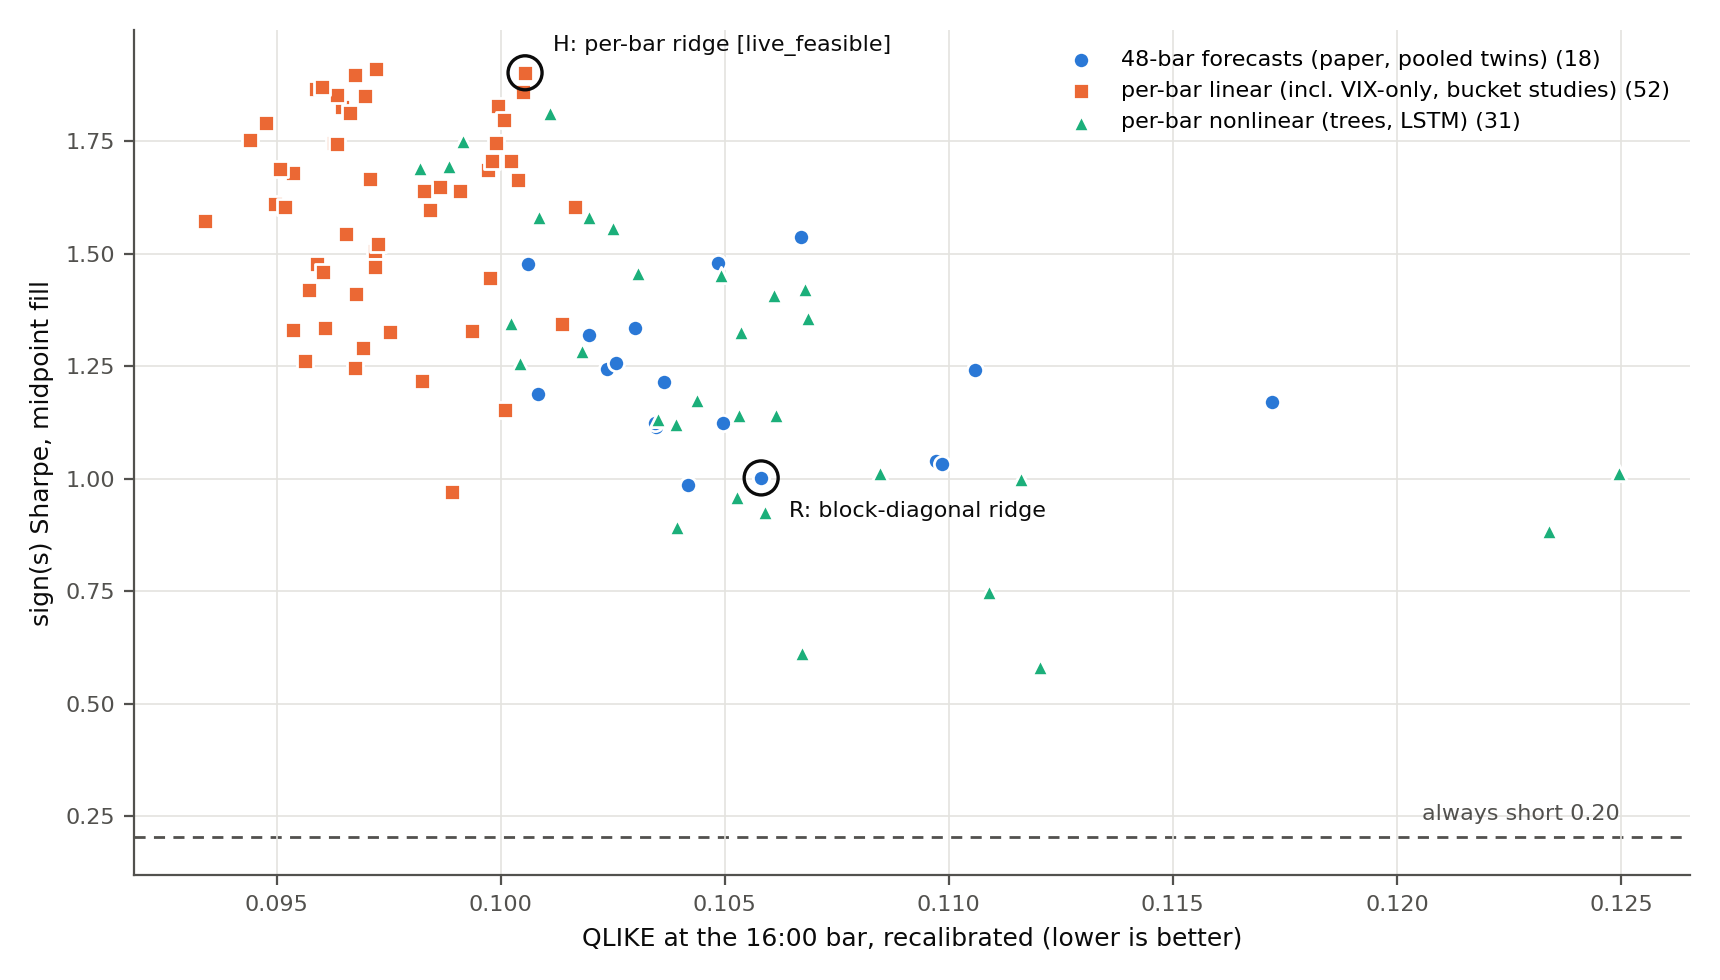
\includegraphics[width=0.85\linewidth]{../results/close_master_table/qlike_vs_sharpe.png}
\caption{Recalibrated 16:00 QLIKE against the sign(s) Sharpe ratio (midpoint fill), table A (check rows and identical forecasts left out); the dashed line is always short. R = reference, H = recommended headline. 5 forecasts lie beyond the plotted QLIKE range (upper quartile + 3 interquartile ranges = 0.126) and are not drawn: per-bar LSTM [all\_features] (QLIKE 0.131, Sharpe 1.33); per-bar LSTM, QLIKE-selected [all\_features] (QLIKE 0.130, Sharpe 1.09); per-bar elastic net [live\_feasible], HAR ladder intra (QLIKE 0.214, Sharpe 0.36); per-bar lasso [live\_feasible], HAR ladder intra (QLIKE 0.218, Sharpe 0.19); per-bar ridge [live\_feasible], HAR ladder intra (QLIKE 0.218, Sharpe -0.02).}
\end{figure}
\end{document}
